\documentclass[
  manuscript=article,
  layout=preprint,
  year=2026,
  volume=x,
]{extra/joas}

% Recent TeX Live releases break the class's numeric author markers (a math-mode marker leaks a font message into
% the author line). The markers are numbers, so they need no math mode.
\makeatletter
\renewcommand*{\cup@author@fnsymbol}[1]{\expandafter\cup@author@fnsymbol@aux\expandafter{\number#1}}
% One author: no "et al." in the running head.
\renewcommand*\cup@etal{}
\makeatother

% Field names of the challenge files
\newcommand{\fld}[1]{\texttt{#1}}
% Ragged-right paragraph column for tables
\usepackage{tabularx}
\newcolumntype{L}[1]{>{\raggedright\arraybackslash}p{#1}}
\usetikzlibrary{arrows.meta,positioning,calc}

% The class prints no DOI, dates, editor or reviewers in the preprint layout; the fields are left empty.
\doi{--}
\received {--}
\revised  {--}
\accepted {--}
\published{--}
\editor{--}
\reviewers{--}

\addbibresource{reference.bib}

\title{Taxi-Out Time as Two Processes: Modelling Schedule Copies in Off-Block Records\footnote{Preprint, not submitted to any journal; set in the JOAS preprint layout for formatting only.}}

\author{Tin Josip Curik}

\keywords{taxi-out time; off-block time; data quality; mixture model; ADS-B}

\abbreviations{
  ADS-B: Automatic Dependent Surveillance--Broadcast,
  CV: cross-validated (score on the January and July 2025 validation folds),
  MSE: mean squared error,
  NM: EUROCONTROL Network Manager,
  RMSE: root mean squared error
}

\hypersetup{pdftitle={Taxi-Out Time as Two Processes: Modelling Schedule Copies in Off-Block Records}}

% Layout note: the class and the logo in its header are the JOAS preprint layout, used for formatting only. The paper has not been submitted
% anywhere and the header is not a claim of acceptance; the page-one footnote on the title says so.
\begin{document}

\begin{abstract}
Taxi-out time, from off-block to take-off, is a basic quantity in the post-operations analysis of airport surface performance.
The EUROCONTROL Performance Review Commission Data Challenge 2026 asked for a prediction of it for every departure at ten European
airports, scored by root mean squared error (RMSE). We show that the label comes from two processes. One is the physical taxi of the
aircraft. The other is the way the record was made: for about one departure in twenty (5.4\% in 2025) the recorded off-block time is
the scheduled time copied into the record, not an observed event, so the label measures the whole delay. On four held-out months, the
741 rows that are such copies, date-stamped records or giant labels carry 46.8\% of the squared error of our final model, and 58.0\%
with the 599 ordinary rows it misses by more than half an hour. We therefore estimate, per departure, the probability that its record
is a schedule copy and predict the probability-weighted mixture of the copy value and a physical taxi estimate, the squared-error
optimum when both parts are calibrated. We measure further record mechanisms on a full year of data and encode them as rules: the
window within which flight plans are attached, date-shifted and duplicated records, and airport-specific stamping regimes. Open ADS-B
ground tracks correct the physical taxi estimate through residual stacking, and EUROCONTROL's published daily delay per airport
constrains each day's sum, never a per-flight value. On two validation months of 2025 the RMSE falls from 660.89\,s for an
airport-mean baseline to 279.61\,s; the three largest gains come from modelling the label, not from a better regressor. A rehearsal,
the whole pipeline rerun with two further months of 2025 hidden, gives 247.48\,s for the reference chain (the final model without its
last additions) against 558.74\,s for the baseline. Two records whose off-block time lies 16 and 23 hours before take-off, with
nothing in their inputs to announce it, carry 36.5\% of the cross-validated squared error of the reference chain; nothing in the
inputs predicts them. The code is open.
\end{abstract}


% ====================================================================================================================
\section{Introduction}
\label{sec:intro}

A departing aircraft leaves its stand (\emph{off-block}), is pushed back, taxis to the runway, waits in the queue of departures and takes
off. How long this takes depends on the route from stand to runway, the traffic that competes for taxiways and runway, the runway
configuration, weather (snow, de-icing, low visibility) and flow regulations that hold a flight at its stand. We call this the
\emph{physical taxi}. Taxi-out time enters airport performance monitoring as additional taxi-out time against an unimpeded reference, and
through it estimates of excess fuel burn and CO$_2$ emissions on the surface. Earlier work predicts it with queuing models of the
departure runway \cite{simaiakis2016queuing}, reinforcement learning \cite{balakrishna2010rl}, statistical and fuzzy regression
\cite{ravizza2014taxi}, and regression trees and neural networks \cite{herrema2018taxi}. These studies take the recorded off-block time as
given and model the physical taxi: distance from stand to runway, queue length, runway configuration and weather.

The EUROCONTROL Performance Review Commission (PRC) Data Challenge 2026 \cite{prc2026challenge} asked participants to predict, for every
departure at ten European airports, the label $y = \fld{MVT} - \fld{BLOCK}$: the recorded take-off time minus the recorded off-block time,
in seconds, scored by RMSE. As in the earlier PRC challenge on take-off weight \cite{spinielli2025tow,murca2025tow}, the setting is
post-operational and the data are open: the challenge files for 2025 (training) and four months of 2026 (test, labels masked), plus any
openly available source.

This paper reports a model for that task and one finding that shapes it: the label comes from two processes (Figure~\ref{fig:flow}).
The first is the physical taxi. The second is the process that writes the record. A person or a system enters the off-block time
\fld{BLOCK}; for most departures it is the observed event, and the label is a taxi of five to twenty-five minutes. For about one
departure in twenty it is the scheduled off-block time copied into the record, and the label then measures the whole delay against the
schedule, sometimes hours. Under squared error these few records dominate the score, and the model's largest gains come from modelling
how the record is produced, not from a better regressor of the physical taxi.

\begin{figure}[htbp!]
  \centering
  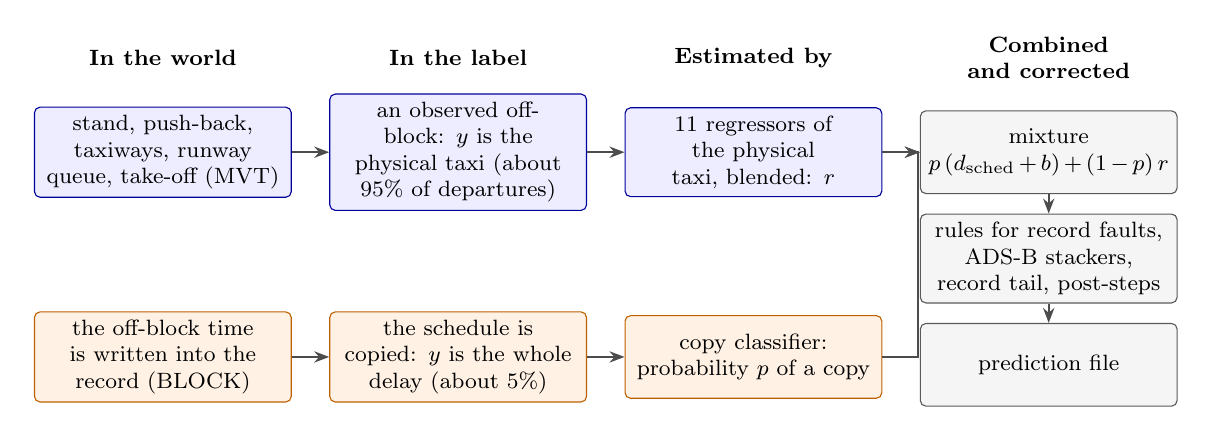
\begin{tikzpicture}[
      font=\footnotesize,
      box/.style={draw, rounded corners=2pt, align=center, text width=3.05cm, minimum height=1.05cm, inner sep=3pt},
      world/.style={box, draw=blue!60!black, fill=blue!7},
      recd/.style={box, draw=orange!75!black, fill=orange!10},
      mdl/.style={box, draw=black!65, fill=black!4},
      head/.style={font=\footnotesize\bfseries, text width=3.2cm, align=center},
      arr/.style={-{Stealth[length=1.9mm]}, thick, black!70}]
    \node[head] at (0,2.5) {In the world};
    \node[head] at (3.75,2.5) {In the label};
    \node[head] at (7.5,2.5) {Estimated by};
    \node[head] at (11.25,2.5) {Combined and corrected};
    \node[world] (p) at (0,1.3) {stand, push-back, taxiways, runway queue, take-off (MVT)};
    \node[recd] (r) at (0,-1.3) {the off-block time is written into the record (BLOCK)};
    \node[world] (py) at (3.75,1.3) {an observed off-block: $y$ is the physical taxi (about 95\% of departures)};
    \node[recd] (ry) at (3.75,-1.3) {the schedule is copied: $y$ is the whole delay (about 5\%)};
    \node[world] (reg) at (7.5,1.3) {11 regressors of the physical taxi, blended: $r$};
    \node[recd] (clf) at (7.5,-1.3) {copy classifier: probability $p$ of a copy};
    \node[mdl] (mix) at (11.25,1.3) {mixture $p\,(d_{\mathrm{sched}}+b) + (1-p)\,r$};
    \node[mdl] (fix) at (11.25,-0.05) {rules for record faults, ADS-B stackers, record tail, post-steps};
    \node[mdl] (out) at (11.25,-1.4) {prediction file};
    \draw[arr] (p) -- (py); \draw[arr] (r) -- (ry);
    \draw[arr] (py) -- (reg); \draw[arr] (ry) -- (clf);
    \draw[arr] (reg) -- (mix); \draw[arr] (clf.east) -- ++(0.45,0) |- (mix.west);
    \draw[arr] (mix) -- (fix); \draw[arr] (fix) -- (out);
  \end{tikzpicture}
  \caption{The label comes from two processes, and the model mirrors them. Top row: the aircraft's physical taxi. Bottom row: the
  record process, which for about one departure in twenty copies the scheduled time instead of observing the event. The regressors
  learn the physical taxi, the classifier learns which records are copies, and the mixture combines the two.}
  \label{fig:flow}
\end{figure}

The contributions are:
\begin{itemize}
  \item a decomposition of the label into a physical taxi and recording artefacts, with each artefact measured on a full year of data
  (Section~\ref{sec:label});
  \item a probabilistic mixture that predicts the conditional mean of the label from a calibrated probability that the record is a
  schedule copy, and a chain of rules, residual models and calibrations around it (Section~\ref{sec:method});
  \item the use of open ADS-B ground tracks to correct the physical taxi, and of a published EUROCONTROL aggregate as a constraint on daily
  sums (Sections~\ref{sec:stackers} and~\ref{sec:calibration});
  \item a validation design for test months without labels from a later year: season-matched folds, a paired day-block bootstrap, a
  rehearsal on two held-out months and a twelve-month score weighted like the test months (Section~\ref{sec:validation}).
\end{itemize}
The model keeps the physical taxi as its own output, so it also reports which records are likely artefacts, which a post-operations
analysis of surface performance needs.

Table~\ref{tb:terms} defines the terms the paper uses, one word per concept.

\begin{table}[htbp!]
  \centering
  \small
  \caption{Terms used throughout. Each row is one term; times are in seconds unless stated.}
  \label{tb:terms}
  \begin{tabular}{L{0.24\textwidth}L{0.68\textwidth}}
  \toprule
  \textbf{Term} & \textbf{Meaning} \\
  \midrule
  label $y$ & take-off time minus recorded off-block time ($\fld{MVT} - \fld{BLOCK}$), the quantity to predict \\
  \fld{BLOCK}, \fld{SCHED}, \fld{MVT} & recorded off-block time, scheduled off-block time, recorded take-off time (Section~\ref{sec:data}) \\
  physical taxi & the time the aircraft really spends between leaving its stand and taking off \\
  copy & a departure whose recorded off-block time equals its scheduled time to within 30\,s, so the label measures the whole delay \\
  copy probability $p$ & the model's estimate that a departure is a copy \\
  member & one of the eleven regressors of the physical taxi; the \emph{blend} is their weighted average \\
  mixture & the prediction $p\,(d_{\mathrm{sched}}+b) + (1-p)\,r$ of Equation~\ref{eq:mixture}: copy value and physical taxi weighted by $p$ \\
  rules, stackers, tail, post-steps & the stages applied after the mixture, in this order: rules for record faults, second-level models of the residual (Section~\ref{sec:stackers}), record tail with the daily-delay calibration, four post-steps and the plan-window step \\
  final model, reference chain & the whole model that produced the submitted file, and the same model without its last additions, on which every step was measured one by one (Section~\ref{sec:results}) \\
  fold, CV & one of two validation months (January and July 2025) with its training months; the cross-validated RMSE on both together \\
  rehearsal & the whole pipeline rerun with two months of 2025 hidden like the test months and scored on them; six rehearsals cover all twelve months, and the two hidden months of one rehearsal are a \emph{held-out pair} \\
  clean and trim rows & rows with label up to 7,200\,s and up to 20,000\,s: the error with and without the heavy tail \\
  \bottomrule
  \end{tabular}
\end{table}


% ====================================================================================================================
\section{Task and data}
\label{sec:data}

\subsection{Task}

The ten airports are Frankfurt (EDDF), Munich (EDDM), London Heathrow (EGLL), Amsterdam (EHAM), Barcelona (LEBL), Madrid (LEMD),
Paris Charles de Gaulle (LFPG), Rome Fiumicino (LIRF), Zurich (LSZH) and Istanbul (LTFM). The training data hold all twelve months of
2025: 4,167,797 movements, of which 2,085,047 are labelled departures. The test data hold 670,790 departures of 2026 with masked labels:
January (152,719), February (144,158), June (181,791) and July (192,122). The score is the RMSE of $y$ in seconds over all test
departures.

\subsection{Challenge data}

Each movement row joins the airport's own record with the NM flight table. The airport record holds the scheduled off-block time
\fld{SCHED}, the take-off time \fld{MVT}, runway, stand, aircraft type, flight number and destination. Where a flight plan exists, the
NM table adds the last filed off-block time \fld{LOBT}, the estimated and initial off-block times \fld{EOBT} and \fld{IOBT}, NM's own
actual off-block time \fld{AOBT\_3}, arrival times at the destination, callsign, operator, market segment and wake category.

Only the departures' \fld{BLOCK} and taxi time are masked in the test files. Arrivals keep their in-block and taxi-in times, so
statistics computed from arrivals are label-free and available at prediction time. Because the task is post-operational, a feature may
read other flights' unmasked records before and after the movement. Every clock enters the model as take-off minus that clock, which
makes each one a candidate taxi time: $d_{\mathrm{aobt}} = \fld{MVT} - \fld{AOBT\_3}$, and likewise $d_{\mathrm{lobt}}$,
$d_{\mathrm{eobt}}$, $d_{\mathrm{iobt}}$ and $d_{\mathrm{sched}}$. For a real off-block event $d_{\mathrm{aobt}}$ is close to the taxi
time.

\subsection{External open data}

Table~\ref{tb:sources} lists the open sources the model reads. None is stored with the code; the pipeline downloads each at run time.
The only input derived from OpenSky Network data \cite{schafer2014bringing} is the OPDI flight-event table \cite{goens2024opdi}.

\begin{table}[htbp!]
  \centering
  \small
  \caption{External open data and their use. Each row is one source.}
  \label{tb:sources}
  \begin{tabular}{L{0.34\textwidth}L{0.58\textwidth}}
  \toprule
  \textbf{Source} & \textbf{Use in the model} \\
  \midrule
  adsb.lol \cite{adsblol} ADS-B history & ground tracks of departures: first heard, first movement, pushback, taxi path, stops \\
  METAR via the Iowa Environmental Mesonet \cite{iem_metar} & weather at the ten airports \\
  EUROCONTROL Performance Review data \cite{ansperformance} & airport-day traffic, ATFM delay by cause, daily pre-departure delay; monthly taxi-out per runway only in a tested step not in the final chain \\
  OPDI flight events \cite{goens2024opdi} & the aircraft's own surface events (taxiway entry, parking exit, runway entry), for 11--13\% of flights \\
  OpenStreetMap \cite{osm}, OurAirports \cite{ourairports} & stand, taxiway and runway geometry \\
  \bottomrule
  \end{tabular}
\end{table}

\subsection{Differences between training and test data}
\label{sec:drift}

Three differences between 2025 and 2026 shape the design. First, seasons differ, so validation uses the same calendar months as the test
set (Section~\ref{sec:folds}). Second, identifiers drift between years: a classifier on label-free features separates all of 2025 from
January and July 2026 at an AUC of 0.968, but January and July 2025 from January and July 2026 only at 0.777 (a control with shuffled
source labels gives 0.501). Of that classifier's feature-importance gain, 46.8\% comes from flight numbers and callsigns, 12.1\% from
stands and 8.7\% from runways, so raw flight numbers and callsigns are not model inputs. Third, take-off times are dithered by a few
seconds in the training files and by about $\pm 12$\,s in the test files, so features measured relative to take-off are rebuilt for each
file and never copied across.


\subsection{Data checks}
\label{sec:checks}

The pipeline makes the following checks on the data it reads; each is a script or a rule in the code (\texttt{code/scripts},
\texttt{code/overnight}). No labelled row is dropped for being extreme: extreme records are sorted into mechanisms
(Section~\ref{sec:mechanisms}) and every test departure receives a prediction.
\begin{itemize}
  \item \textbf{Impossible stand durations.} The label-free stand-level averages of $\mathrm{take\text{-}off} - \fld{AOBT\_3}$ use only
  values from 0 to 3,600\,s; others are treated as missing before the average is formed.
  \item \textbf{Off-block far from take-off.} When take-off minus \fld{AOBT\_3} exceeds 20,000\,s the record is date-shifted (NM
  off-block, \fld{EOBT} and \fld{BLOCK} a day early) and the prediction is that difference.
  \item \textbf{Local midnight.} The Rome date-stamp record requires the take-off to fall on a later local (Europe/Rome) date than the
  schedule; this held in all 12 such cases of 2025.
  \item \textbf{Duplicated records.} Two records of one take-off (mostly LFPG, 118 pairs) are found; only the NM-matched half tracks the
  plan.
  \item \textbf{Consistency with the flight plan.} $|\fld{BLOCK} - \fld{LOBT}| \le 3{,}606$\,s holds in all 2,062,577 planned departures
  of 2025, and the plan window built on it is applied to the test files.
  \item \textbf{ADS-B take-off.} A departure counts as matched only when the ADS-B take-off (the first point at 90 knots or more) lies
  within 300\,s of its recorded take-off.
  \item \textbf{Raw ADS-B days} (\texttt{validate\_days.py}). A day file is rejected when it cannot be read, a partial file sits next to
  it, it has fewer than 0.4 times the median row count of the days within three days of it, or one of the ten airports has no rows
  while its neighbours do.
  \item \textbf{Feature coverage} (\texttt{final\_coverage.py}). For each feature file and test month the non-missing share must reach
  0.8 times that of the same calendar month in training.
  \item \textbf{Prediction file} (\texttt{validate\_file.py}, \texttt{check\_final.py}). Exactly the template's columns, its ids in order
  and unique, finite non-negative seconds, every step of the model traceable to a recorded configuration, and a recorded checksum of
  the final file.
\end{itemize}


% ====================================================================================================================
\section{The label is two processes}
\label{sec:label}

\subsection{Schedule copies}

Most departures taxi for five to twenty-five minutes. For about 5\% of departures the recorded \fld{BLOCK} is not an event: it is the
scheduled time copied into the record. We call such a record a \emph{copy} when $|\fld{BLOCK} - \fld{SCHED}| \le 30$\,s. Its label is
then $y = \fld{MVT} - \fld{SCHED} = d_{\mathrm{sched}}$, the whole delay against the schedule. Figure~\ref{fig:timeline} shows both cases.
Copies make up 5.4\% of the 2025 departures and between 4.6\% and 6.2\% in every month. Their share depends on the airport (18\% at LIRF,
3--6\% elsewhere) and, at LIRF, strongly on the carrier (4--55\% among its large carriers, 1.5--7\% elsewhere), which points to the
handler who stamps the record rather than to operations.

\begin{figure}[htbp!]
  \centering
  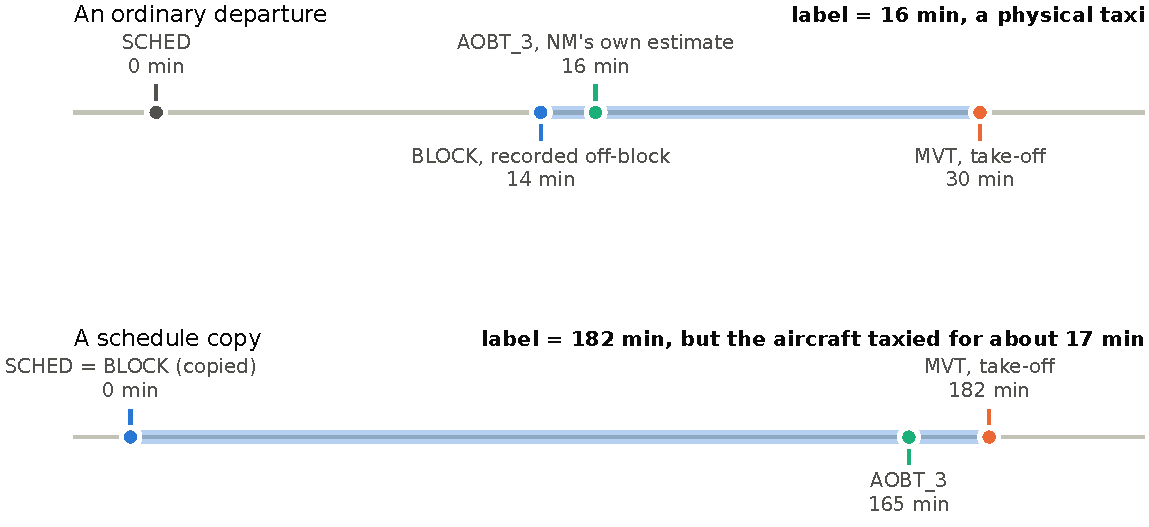
\includegraphics[width=0.95\textwidth]{figures/fig-timeline.pdf}
  \caption{One departure, two ways to record it. Top: the record holds the push-back and the label is the taxi. Bottom: the record
  holds the schedule, and the label counts the whole delay as taxi.}
  \label{fig:timeline}
\end{figure}

Table~\ref{tb:regimes} and Figure~\ref{fig:regimes} split the cross-validated error of the model by label regime. Ordinary taxis are
94.75\% of the rows and carry 41.6\% of the squared error; copies are 5.07\% and carry 13.1\%; 52 records over two hours that are not
copies carry 40.2\%.

\begin{table}[htbp!]
  \centering
  \small
  \caption{Rows and squared error by label regime, for the reference chain (CV 285.44\,s, Section~\ref{sec:results}) on the 344,419
  validation departures of the two folds. Each row is one regime of the label; \emph{Rows} counts its departures, \emph{Squared error} is
  its share of the total squared error, \emph{RMSE} its own root mean squared error and \emph{Mean error} its mean of prediction minus truth.}
  \label{tb:regimes}
  \begin{tabular}{lrrrrr}
  \toprule
  \textbf{Label regime} & \textbf{Rows} & \textbf{Rows (\%)} & \textbf{Squared error (\%)} & \textbf{RMSE (s)} & \textbf{Mean error (s)} \\
  \midrule
  physical taxi up to 1\,h & 326,333 & 94.75 & 41.6 & 189.2 & $+3.4$ \\
  schedule copy & 17,450 & 5.07 & 13.1 & 459.7 & $-98.0$ \\
  1--2\,h, not a copy & 584 & 0.17 & 5.0 & 1,553.4 & $-991.5$ \\
  over 2\,h, not a copy & 52 & 0.02 & 40.2 & 14,732.6 & $-5{,}571.1$ \\
  \bottomrule
  \end{tabular}
\end{table}

\begin{figure}[htbp!]
  \centering
  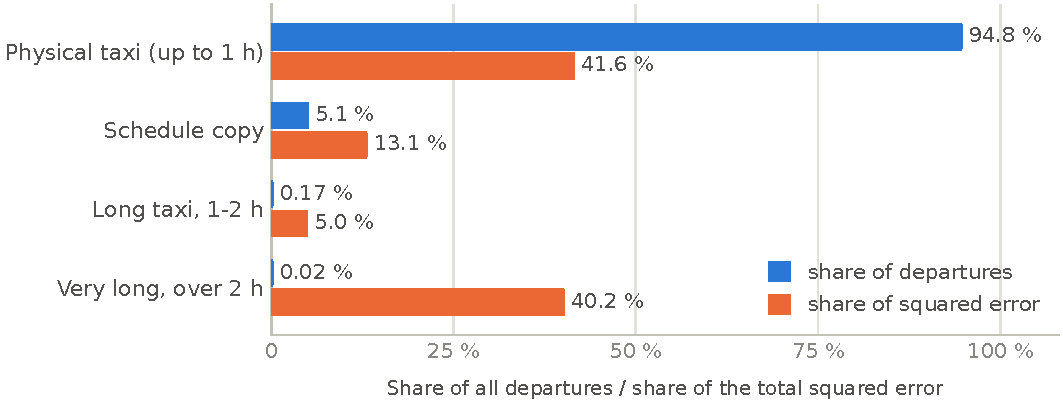
\includegraphics[width=0.85\textwidth]{figures/fig-regimes.pdf}
  \caption{Share of departures and of squared error by label regime. 95\% of the rows are ordinary taxis and carry 42\% of the squared
  error; 52 records over two hours carry 40\%.}
  \label{fig:regimes}
\end{figure}

\subsection{Concentration of the error}
\label{sec:concentration}

The squared error is extremely concentrated (Figure~\ref{fig:concentration}): 2 rows carry 36.5\% of it, 10 rows 42.1\%, 100 rows
51.1\% and 1,000 rows 64.1\%. The two largest errors are LFPG departures from January 2025 without an NM flight plan. They took off 29 and
34 minutes after schedule, which looks ordinary, yet their recorded off-block lies 23.4\,h and 16.2\,h before take-off (labels 84,240\,s
and 58,206\,s), and nothing in their inputs points to it. Without these two rows the cross-validated RMSE of the reference chain would be
227.44\,s instead of 285.44\,s. Every comparison in this work is therefore also reported on \emph{trim} rows (label up to 20,000\,s,
about 5.5\,h) and \emph{clean} rows (label up to 7,200\,s), so that a gain can be checked with and without the heavy tail.

\begin{figure}[htbp!]
  \centering
  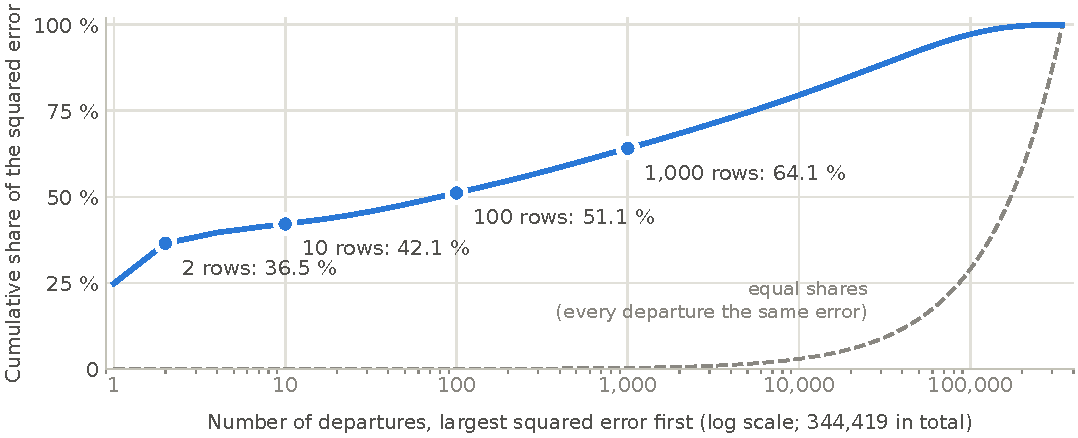
\includegraphics[width=0.85\textwidth]{figures/fig-concentration.pdf}
  \caption{Cumulative share of the squared error, departures sorted by squared error. Two departures carry 36.5\% of it and the first
  hundred 51.1\%; the dashed line is the curve if every departure had the same error.}
  \label{fig:concentration}
\end{figure}

\subsection{How the recorded off-block goes wrong}
\label{sec:mechanisms}

Table~\ref{tb:mechanisms} lists the mechanisms that produce large labels. Each was measured on the 2025 training data, and each is a
component of the model. Two of them bound the label rather than add to it: an NM flight plan is attached to a departure record only when
$|\fld{BLOCK} - \fld{LOBT}| \le 3{,}606$\,s, which holds in all 2,062,577 departures of 2025 that have a plan; and no departure whose last
filed off-block lies more than an hour after schedule is a copy (0 of 66,025), against 69 copies in the 60\,s bin just below that
threshold. Re-filing the plan evidently replaces the copied stamp with a real one.

\begin{table}[htbp!]
  \centering
  \small
  \caption{Record mechanisms, their evidence in the 2025 data and their use in the model. Each row is one way the recorded off-block goes wrong.}
  \label{tb:mechanisms}
  \begin{tabular}{L{0.25\textwidth}L{0.4\textwidth}L{0.27\textwidth}}
  \toprule
  \textbf{Mechanism} & \textbf{Evidence in 2025} & \textbf{Use in the model} \\
  \midrule
  Schedule copy: \fld{BLOCK} is the scheduled time & 5.4\% of departures (4.6--6.2\% per month); LIRF 18\%, other airports 3--6\% & copy classifier and mixture \\
  Plan cliff: $\fld{LOBT} - \fld{SCHED} > 3{,}600$\,s & 0 copies among 66,025 such departures & copy probability set to 0 \\
  Plan window & $|\fld{BLOCK} - \fld{LOBT}| \le 3{,}606$\,s in all 2,062,577 planned departures & prediction clipped to $d_{\mathrm{lobt}} \pm 3{,}606$\,s \\
  Date-shifted record: NM off-block, \fld{EOBT} and \fld{BLOCK} a day before take-off & e.g.\ $d_{\mathrm{aobt}} = 87{,}181$\,s, label 87,002\,s & $d_{\mathrm{aobt}} > 20{,}000$\,s $\Rightarrow$ predict $d_{\mathrm{aobt}}$ \\
  Gate hold: NM off-block far after \fld{LOBT}, handler stamp near \fld{LOBT} & 151 validation rows & prediction moved halfway to $d_{\mathrm{lobt}}$ \\
  LIRF long copy: no plan, take-off over 20,000\,s after schedule & 48 of the 50 at 20,000--50,000\,s are copies & predict $d_{\mathrm{sched}}$ \\
  LIRF date stamp: schedule's local date plus the true off-block time of day & 12 rows, all with take-off on a later Rome date & label $\approx 86{,}400$\,s plus taxi \\
  LIRF near-schedule group: two carriers' no-plan departures within 1\,h of schedule & 17 of 20 labels in 7.7--8.3\,ks & the group's 2025 mean \\
  Duplicated take-off records (mostly LFPG) & 118 pairs; the NM-matched half tracks $d_{\mathrm{lobt}}$ (correlation 0.94) & linear rule on the matched half \\
  \bottomrule
  \end{tabular}
\end{table}

A taxonomy of every 2025 departure with a label above 3,600\,s or below zero (4,495 rows, of which 4,173 are itemised) sizes the
mechanisms by the squared error a flat 900\,s prediction would make on them: schedule copies carry 53\% of that cost (1,797 rows), records
with \fld{BLOCK} a day early 31\% (13 rows), one record at $\fld{SCHED} - 24$\,h 2\%, about 240 hour-shifted or exact copies of
\fld{AOBT\_3}, \fld{LOBT} or \fld{EOBT} 1\%, and 2,122 unexplained rows 13\%, of which 2,001 are genuine taxis of one to two hours.


% ====================================================================================================================
\section{Method}
\label{sec:method}

\subsection{Overview}

Figure~\ref{fig:pipeline} shows the model. A classifier estimates the probability $p$ that a departure's recorded off-block is a copy of
its schedule; eleven members estimate the physical taxi; the two are mixed. A chain of rules for known record faults follows, then
second-level models that correct the residual from ADS-B tracks, a tail of record rules and a calibration to a published aggregate, four
post-steps for mechanisms the stack still misses, and a final consistency step. Each stage reads the previous stage's out-of-fold predictions, made by models that never saw that row's month.

\begin{figure}[htbp!]
  \centering
  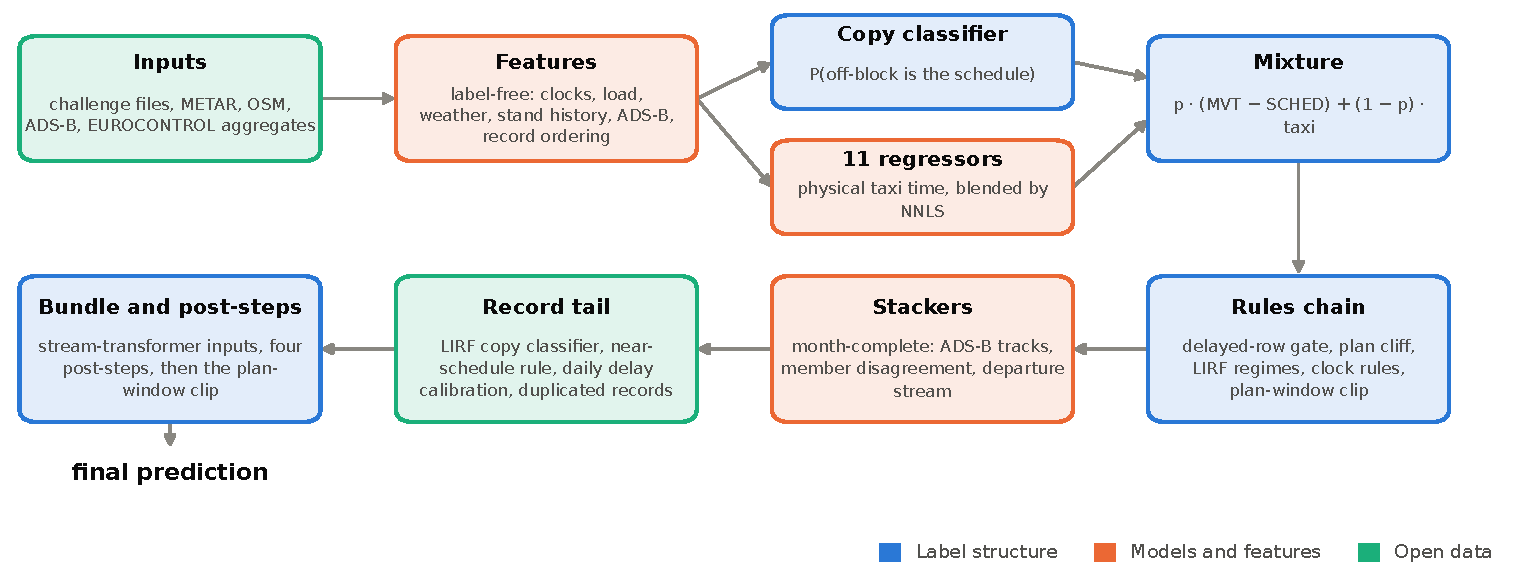
\includegraphics[width=\textwidth]{figures/fig-pipeline.pdf}
  \caption{The model. Top row: inputs, features, the copy classifier and the regressors, the mixture. Bottom row, right to left: the
  corrections applied after the mixture, in order. Colours mark the stage's family: label structure, models and features, open data.}
  \label{fig:pipeline}
\end{figure}

\subsection{The mixture}
\label{sec:mixture}

Let $c$ indicate a copy. By the law of total expectation,
\begin{equation} \label{eq:total}
\mathrm{E}[y \mid x] = P(c \mid x)\,\mathrm{E}[y \mid c, x] + \bigl(1 - P(c \mid x)\bigr)\,\mathrm{E}[y \mid \neg c, x].
\end{equation}
For a copy, $y = d_{\mathrm{sched}}$ up to the 30\,s tolerance, so $\mathrm{E}[y \mid c, x] = d_{\mathrm{sched}} + b$, with $b$ the
mean of $y - d_{\mathrm{sched}}$ over training copies (about zero). With $p$ an estimate of $P(c \mid x)$ and $r$ a regressor fitted on
non-copy rows, the prediction is
\begin{equation} \label{eq:mixture}
\hat{y} = p\,(d_{\mathrm{sched}} + b) + (1 - p)\,r .
\end{equation}
Since the conditional mean minimises the expected squared error, Equation~\ref{eq:mixture} is the squared-error optimum when $p$ and $r$
are calibrated. Figure~\ref{fig:mixture} illustrates it for a departure with a 30\% copy probability, a physical taxi
of 15 minutes and 180 minutes since schedule: the expected cost is minimised at 64.5 minutes, between the two answers, and either answer
alone costs more.

The calibration of $p$ matters more than its ranking. A copy missed on a flight that left three hours late costs about $10^8$\,s$^2$, so
a probability of 30\% must mean 30\%. Gates that try to single out the rows with huge errors instead do not beat this conditional mean.

\begin{figure}[htbp!]
  \centering
  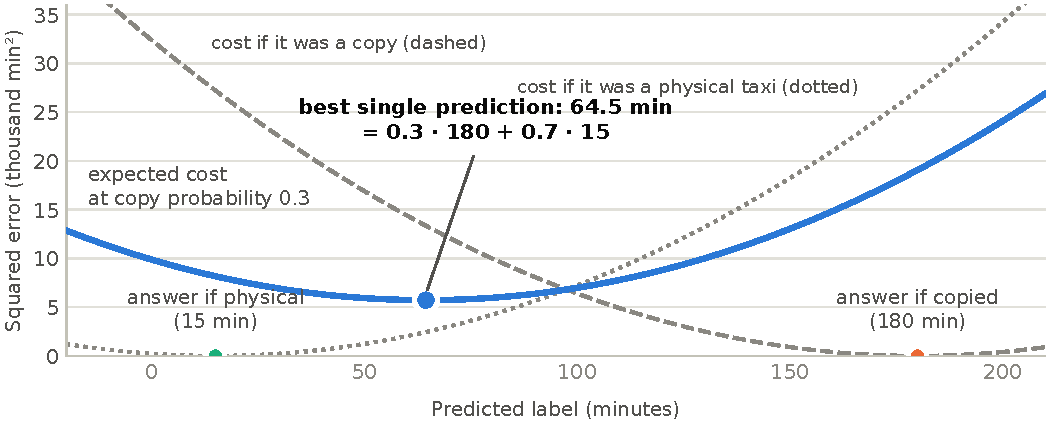
\includegraphics[width=0.85\textwidth]{figures/fig-mixture.pdf}
  \caption{Expected squared error against the prediction for a departure with a 30\% copy probability (physical taxi 15\,min, 180\,min
  since schedule). The weighted mix has a lower expected cost than either answer alone.}
  \label{fig:mixture}
\end{figure}

\subsection{Copy classifier}
\label{sec:copyclf}

The copy probability comes from an XGBoost classifier \cite{chen2016xgboost} (depth 8, learning rate 0.05, minimum child weight 5,
subsample 0.8, column sample 0.7), early-stopped on log loss. It reads challenge data only: the clocks, the recording process (whether an
NM plan matched, mismatches between the airport and NM records, airline, stand prefix), arrival-side copy habits, surface load and stand
and runway history (Section~\ref{sec:features}). Out of fold on the two validation folds (344,419 departures, 5.07\% copies), $p$ is
close to calibrated without post-hoc scaling (Table~\ref{tb:copyclf}, Figure~\ref{fig:reliability}). It under-predicts slightly overall
(4.80\% against 5.07\%) and in the bins above 10\%, and over-predicts the large bin of near-certain non-copies (0.31\% against 0.19\%).
The largest gap, 3.9 percentage points, falls in a bin of 583 rows.

\begin{table}[htbp!]
  \centering
  \small
  \caption{Out-of-fold quality of the copy probability on the validation departures; each row is a subset of them. \emph{Copy share} is the
  observed share of copies, \emph{Mean $p$} the mean predicted probability; log loss and Brier score \cite{brier1950verification} are
  lower for a better probability, AUC higher; values in brackets are a constant prediction at the base rate.}
  \label{tb:copyclf}
  \begin{tabular}{lrrllr}
  \toprule
  \textbf{Rows} & \textbf{Copy share} & \textbf{Mean $p$} & \textbf{Log loss} & \textbf{Brier} & \textbf{AUC} \\
  \midrule
  all & 5.07\% & 4.80\% & 0.148 (0.200) & 0.041 (0.048) & 0.870 \\
  January fold & 5.62\% & 5.66\% & 0.163 (0.216) & 0.045 (0.053) & 0.861 \\
  July fold & 4.62\% & 4.10\% & 0.136 (0.187) & 0.037 (0.044) & 0.879 \\
  LIRF only & 16.7\% & 16.2\% & 0.309 (0.452) & 0.096 (0.139) & 0.866 \\
  \bottomrule
  \end{tabular}
\end{table}

\begin{figure}[htbp!]
  \centering
  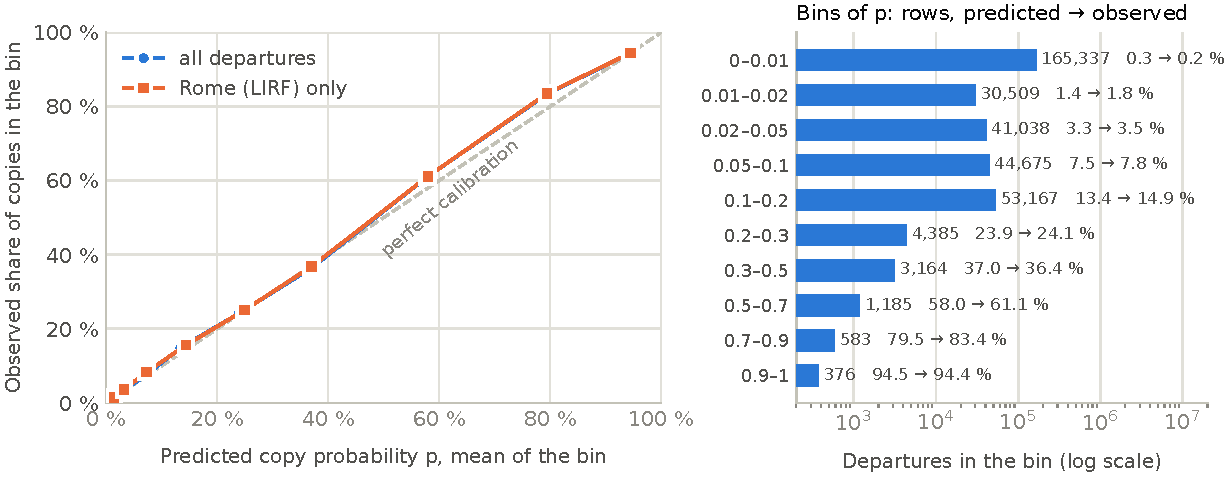
\includegraphics[width=\textwidth]{figures/fig-copy-reliability.pdf}
  \caption{Reliability of the copy probability, out of fold. Left: observed copy share against the mean predicted probability in ten
  bins, for all departures and for LIRF alone. Right: rows per bin with predicted and observed share.}
  \label{fig:reliability}
\end{figure}

\subsection{Features}
\label{sec:features}

No departure's own \fld{BLOCK} or taxi time feeds its features. Two feature families are outputs of models trained on labels (the
month-complete ADS-B model and the member-disagreement features below); both are out-of-month. Statistics that use labels are fitted on
training months only, or month-out-of-fold. Table~\ref{tb:features} summarises the families and their operational reasons.

\begin{table}[htbp!]
  \centering
  \small
  \caption{Feature families and their operational reasons. Each row is one family; the \emph{Reason} is the mechanism it stands for.}
  \label{tb:features}
  \begin{tabular}{L{0.2\textwidth}L{0.36\textwidth}L{0.36\textwidth}}
  \toprule
  \textbf{Family} & \textbf{Content} & \textbf{Reason} \\
  \midrule
  Clocks & take-off minus \fld{AOBT\_3}, \fld{LOBT}, \fld{EOBT}, \fld{IOBT}, \fld{SCHED}; gaps between clocks & $d_{\mathrm{aobt}}$ is an independent off-block estimate; gaps measure re-planning, and copies occur where nobody re-planned \\
  Recording process & NM plan matched, record mismatches, airline, stand prefix & the way the off-block is recorded (plan matched or not, which airline) decides whether it is an event or a copy of the schedule \\
  Arrival-side copy habits & share of the airline's or airport's arrivals whose in-block equals schedule; previous arrival at the stand & arrivals are not masked; departures are copies in 13.2\% of cases when the stand's previous arrival was one, 5.2\% otherwise \\
  Surface load & departures and arrivals around take-off and during the taxi, per airport and runway; queue at take-off & taxi time grows with the aircraft competing for taxiways and runway \\
  Stand and runway history & taxi-in at the same stand; other departures' $d_{\mathrm{aobt}}$ at the same stand and stand--runway pair & stand-to-runway distance and routing are stable, so earlier taxis from the same stand and pair predict the next one \\
  Geometry & stand position, taxi-network and straight-line distance to the runway threshold & the physical length of the taxi \\
  Weather (METAR) & snow, freezing and de-icing conditions, thunderstorms, low visibility, wind, temperature & de-icing after off-block and low-visibility procedures lengthen the taxi \\
  Network and ATFM & airport-day traffic, ATFM delay by cause, regulated share, slot adherence & a regulated day changes stand and runway sequencing \\
  Record ordering and backlog & record id against neighbours in take-off order; flights past \fld{EOBT} not yet off-block & a low id for its slot marks a flight that left late against its plan \\
  Own-flight events (OPDI) & take-off minus taxiway entry, parking exit, runway entry & a direct observation of the taxi where it exists, which replaces the estimate for those flights \\
  ADS-B ground track & first heard, first movement, roll start, end of last stop, stops, path length; pushback detection & where the recorded off-block is a copy, the first movement and the start of the roll still bound the physical taxi \\
  Departure-stream context & label-free aggregates of the airport's other departures around the flight & departures close in time share queue, runway and weather conditions that no per-flight field records \\
  \bottomrule
  \end{tabular}
\end{table}

The ADS-B track of a departure is found by callsign within $\pm 90$ minutes of take-off; a departure is \emph{matched} when an ADS-B
take-off lies within 300\,s of its recorded take-off. Most aircraft are first heard after off-block (median $+225$\,s, transponders are
off at the stand), so the track cannot say when the aircraft left the stand, only when it moved. Pushback is detected as reverse motion:
consecutive fixes under 60\,s and 2--150\,m apart whose bearing differs from the reported heading by more than 135$^\circ$.

\subsection{Regressors and blend}
\label{sec:regressors}

Each member fits non-copy rows only. Its target is the label minus a clock-based guess, the \emph{anchor}, so it learns a correction
rather than the whole taxi. The \fld{AOBT\_3} anchor is $\mathrm{clip}(d_{\mathrm{aobt}}, 0, 3600)$, with the median filling a missing
value; the \fld{LOBT} anchor is $d_{\mathrm{lobt}}$ on planned rows, falling back to the \fld{AOBT\_3} anchor. Because $|\fld{BLOCK} -
\fld{LOBT}|$ is bounded by the plan window, the \fld{LOBT} anchor has no heavy tail. The training residual is clipped at $\pm 5{,}000$\,s
so that rare multi-hour non-copy rows do not steer the fit.

Eleven members (regressors of the physical taxi) differ in learner (CatBoost \cite{prokhorenkova2018catboost}, multilayer perceptrons with four layers of 1,024 units,
and a denoising autoencoder with swap noise \cite{vincent2008dae} and a regression head), anchor and input set (Table~\ref{tb:members}).
All members share the classifier's $p$; only the regressor branch is blended, $\hat{y} = p\,(d_{\mathrm{sched}} + b) + (1-p) \sum_i
w_i r_i$, with non-negative least squares (NNLS) weights \cite{lawson1974nnls} fitted on pooled out-of-fold predictions of non-copy rows.
The weights are cross-fitted (fitted on January and applied to July, and the reverse), so the optimism of fitting eleven weights on the
validation folds (0.44\,s) is not in any reported number. Per-airport weights do not improve the blend.

\begin{table}[htbp!]
  \centering
  \small
  \caption{The eleven members. The \emph{base set} is the challenge-data features (clocks, recording process, arrival habits, load,
  stand and runway history, record ordering). Each row is one member. \emph{CV alone} is the member's RMSE as the only regressor in the mixture, before any rule; \emph{Weight} is its weight in the blend.}
  \label{tb:members}
  \begin{tabular}{rllL{0.36\textwidth}rr}
  \toprule
  \textbf{\#} & \textbf{Learner} & \textbf{Anchor} & \textbf{Inputs beyond the base set} & \textbf{CV alone} & \textbf{Weight} \\
  \midrule
  1 & CatBoost & LOBT & weather, EUROCONTROL, OSM, OPDI, ordering, ADS-B & 429.79 & 0.198 \\
  2 & MLP & LOBT & ADS-B & 433.38 & 0.219 \\
  3 & CatBoost (seed 2) & AOBT & as 1 & 436.00 & 0.121 \\
  4 & MLP & AOBT & as 1 & 437.40 & 0.214 \\
  5 & CatBoost & AOBT & as 1 & 437.58 & 0.174 \\
  6 & CatBoost & LOBT & weather, EUROCONTROL, OSM, OPDI, ordering & 437.63 & 0.036 \\
  7 & CatBoost & AOBT & weather, EUROCONTROL, OSM, OPDI, ordering & 444.73 & 0 \\
  8 & CatBoost, depth 10 & AOBT & weather, EUROCONTROL, OSM, OPDI & 446.41 & 0 \\
  9 & CatBoost, 16k iterations & AOBT & none & 446.47 & 0 \\
  10 & MLP & AOBT & none & 449.05 & 0 \\
  11 & DAE + MLP head & AOBT & none & 455.22 & 0.036 \\
  \bottomrule
  \end{tabular}
\end{table}

The blend gains little over the best member (429.50 against 429.79). The members earn their place later: their disagreement is an input
of the residual stackers worth $-0.84$\,s of RMSE (Section~\ref{sec:stackers}), and that needs members that differ in learner and
anchor, including those with weight zero in the blend.

\subsection{Rules chain}
\label{sec:rules}

Five rules follow the blend (Table~\ref{tb:rules}). The \emph{delayed-row gate} addresses the fact that copies are expensive only on
delayed rows, where a miss costs about $d_{\mathrm{sched}}^2$: a CatBoost classifier $q$ of the same copy flag, fitted only on
departures 900--20,000\,s late and cross-fitted by month, is mixed into the copy probability as $p + w\,(q - p)$, with $w = 0.75$ at LIRF
and zero elsewhere, because at LIRF the copy share follows the handler and stays flat across months while genuine delays grow with
summer traffic; $q$ is averaged over five seeds because GPU CatBoost is not bit-reproducible. The \emph{plan cliff} sets $p = 0$ when
$\fld{LOBT} - \fld{SCHED} > 3{,}600$\,s. The \emph{LIRF regimes} assign LIRF departures without a plan and with a large
$d_{\mathrm{sched}}$ to a copy ($y = d_{\mathrm{sched}}$), a date stamp ($y = 86{,}400\,\mathrm{s}$ plus taxi, only across a local
midnight) or a real taxi, with rates per cell fitted on each fold's training months only. The \emph{clock rules} encode the date-shifted
record, the gate hold and the LIRF long copy of Table~\ref{tb:mechanisms}, and the \emph{plan-window clip} keeps planned rows within
$d_{\mathrm{lobt}} \pm 3{,}606$\,s.

\begin{table}[htbp!]
  \centering
  \small
  \caption{CV RMSE (s) after each rule is added to the rows above it, out of fold. \emph{Jan} and \emph{Jul} are the RMSE on each fold.}
  \label{tb:rules}
  \begin{tabular}{lrrr}
  \toprule
  \textbf{After} & \textbf{CV} & \textbf{Jan} & \textbf{Jul} \\
  \midrule
  blend mixture & 429.50 & 378.42 & 466.61 \\
  + delayed-row gate & 426.87 & 377.71 & 462.71 \\
  + plan cliff & 426.50 & 377.01 & 462.55 \\
  + LIRF regimes & 295.88 & 327.65 & 267.54 \\
  + clock rules & 292.41 & 326.81 & 261.41 \\
  + plan-window clip & 292.33 & 326.80 & 261.27 \\
  \bottomrule
  \end{tabular}
\end{table}

The LIRF regimes carry almost all of the gain ($-130.6$\,s): at Rome the long no-plan rows are copies or date stamps, and the mixture
alone cannot reach those values.

\subsection{Residual stackers}
\label{sec:stackers}

A stacker \cite{wolpert1992stacked} is a second-level model that predicts the residual $y - \hat{y}$ the chain still makes; its
prediction is added back. Its inputs are the ADS-B timings, stops and path; the chain's own prediction and the clock gaps; the airport;
a month-complete ADS-B model (a taxi-time prediction from ADS-B and clocks for every month of 2025, each month predicted from the other
eleven); pushback features; and the members' disagreement (each member's gap to the blend, their spread and range). Rows without an ADS-B
match are corrected by a second model of the same learner from clocks and the chain prediction. The fit uses non-copy rows with
$y \le 20{,}000$\,s and a residual clipped at $\pm 1{,}800$\,s; LIRF rows train the model but are not corrected. Cross-fitting uses five
day-blocks over both validation months with three seeds.

Four stackers are averaged with equal weights (Table~\ref{tb:stackers}): XGBoost, CatBoost, LightGBM \cite{ke2017lightgbm} with extremely
randomised trees, and XGBoost with rows weighted to the ADS-B coverage mix of 2026. That weighting exists because coverage in the
validation months differs strongly from the same months of 2026 (LEMD January 0\% to 97\%, EGLL July 27\% to 98\%, EDDF 91--94\% to
73--74\%). Cross-fitted NNLS weights over the four stackers add nothing over the equal average. The member-disagreement inputs gain
$-0.84$\,s [$-1.11$, $-0.65$] on the folds and $-0.50$\,s [$-0.84$, $-0.22$] on the held-out rehearsal months of
Section~\ref{sec:rehearsal}.

\begin{table}[htbp!]
  \centering
  \small
  \caption{CV RMSE (s) of the chain after each residual stacker. Each row is one stacker used alone; the last row averages the four.}
  \label{tb:stackers}
  \begin{tabular}{lr}
  \toprule
  \textbf{Stacker} & \textbf{CV after} \\
  \midrule
  XGBoost, depth 7 & 289.08 \\
  CatBoost & 288.97 \\
  LightGBM, extra trees, 127 leaves & 289.00 \\
  XGBoost, rows weighted to 2026 ADS-B coverage & 289.50 \\
  equal average & 288.85 \\
  \bottomrule
  \end{tabular}
\end{table}

Two additions over this \emph{reference chain}, and two inputs from a stream transformer described below, complete the final model. \emph{Departure-stream context} adds label-free
aggregates of the airport's other departures around each flight (mean delay against schedule and plan, overdue backlog, throughput
against the airport-hour norm, arrival delay, neighbours' predictions) to the stackers' inputs. \emph{Month-complete stackers}
train on the January and July out-of-fold rows plus five further rehearsals, each hiding two months of 2025 (February and June, March
and September, April and October, May and November, August and December) and producing honest out-of-month base predictions for its
pair (1.74 million rows in total). In each rehearsal the stacker learns from the other pairs only, never from the pair it is scored on.

A stacker trained on two months has seen the airport only in January and July; asked about a March flight, it extrapolates from
seasons it knows. With the five rehearsals it has seen every season of the year with
honest, out-of-month errors of the chain, so what it learns (when a ground track says the base prediction is too long, how a clock gap
turns into delay) holds across the year, and it is scored on a pair of months whose rows it never trained on.

The last inputs come from a \emph{stream transformer}. A queue at a runway belongs to the stream of aircraft, not to any
one of them, so every movement of an airport, departures and arrivals, becomes a token in time order, with its clocks, plan and features.
A transformer over chunks of 512 tokens lets each departure attend to the flights around it; a learned decay per attention head sets how
far back each head looks. One network, the \emph{track-aware network}, is trained with ADS-B modality dropout (the track block
of some tracked departures is hidden, so it also predicts untracked ones) and with self-distillation from an averaged copy of itself
that sees the full chunk; its output becomes five stacker columns (its prediction, its gap to the chain, its spread, and the
probabilities that the label exceeds 1,800 and 3,600\,s). A second network, the \emph{context network}, has the departure-stream windows on each
departure token and joins the member-disagreement inputs. Both also reconstruct masked inputs on the label-free input streams of the
months they predict; neither reads a label of those months.

The final variant adds a head that predicts the level of the queue a departure shares with its neighbours: its target is the
leave-one-out mean of the clipped residuals of the other labelled departures of the same airport and of the same runway within $\pm 30$ minutes,
shrunk towards zero where few neighbours exist, and built inside each fit from that fit's own training months, so a validation month never sees its
own labels and the test months get no label target. Its two extra columns join the track-aware network's five. On the twelve months weighted like the test months, over six month
pairs, month-complete stackers with both inputs against the reference chain with departure-stream context gain $-1.67$\,s [$-1.88$, $-1.45$]; the neighbour-label head alone, against the same
stackers without it, gains $-0.13$\,s [$-0.20$, $-0.06$] and improves 11 of the 12 months.

\subsection{Record tail and calibration to published aggregates}
\label{sec:calibration}

After the stackers, a tail of steps handles specific record faults (Table~\ref{tb:tail}). A LIRF no-plan copy classifier (CatBoost,
trained across all twelve months out-of-fold) is applied with weight 0.5 to ADS-B-matched LIRF departures without an NM off-block that
took off 1--5.6\,h after schedule. A LIRF near-schedule rule sets two carriers' no-plan departures within an hour of schedule to the
group's mean 2025 label. A duplicated-record rule predicts the NM-matched half of a duplicated take-off record as $a + b\,d_{\mathrm{lobt}}$,
with $a$ and $b$ fitted by least squares on 2025 pairs outside the scored month ($a = 120$\,s, $b = 0.90$ on all of 2025).

EUROCONTROL publishes aggregates computed from the same off-block records the label is built from. The final chain uses one of them,
the daily delay, as a constraint on a total, never as a per-row value; a second, the monthly runway taxi-out, was tested and left out.

\paragraph{Daily delay.} The published daily all-cause pre-departure delay per airport, $D_{a,t}$ (per UTC day $t$ of take-off), equals
\begin{equation} \label{eq:daily}
D_{a,t} = \sum_{i \in (a,t)} \max(\fld{BLOCK}_i - \fld{SCHED}_i, 0) = \sum_{i \in (a,t)} \max(d_{\mathrm{sched},i} - y_i, 0)
\end{equation}
on 2025 (correlation 0.9997, median ratio 1.000). For each airport-day we solve one multiplicative factor on the ordinary rows (prediction below
3,600\,s) that makes the total implied by the predictions in Equation~\ref{eq:daily} equal the published one, and apply 0.6 of that
change. A day without a published value stays unchanged.

\paragraph{Monthly runway taxi-out (tested, not in the final chain).} EUROCONTROL publishes the mean taxi-out per airport, runway and month for valid flights only
(taxi-out up to 120 minutes, de-iced flights removed) and the share of flights counted as invalid. A cell's label mean differs from the
published mean by an offset, mostly the excluded flights. The step models that offset as the cell's mean over the other 2025 months plus
a per-airport slope times the month's invalid share, and moves rows owned by the regressors a quarter of the way towards the published mean
plus offset, by at most 150\,s per cell. Cells whose invalid share lies outside the 2025 range are left alone, as is January at the four
airports that de-ice after off-block (EDDF, EDDM, LFPG, LSZH). Skipping February there as well scored worse (twelve-month
leave-one-month-out: February's gain 60 instead of 67 MSE; held-out February 2025 rehearsal: 8 MSE worse), so February is kept. The
step gains $-0.03$\,s on the folds and in every held-out pair (6 of 6). The final chain leaves it out, so that it uses one published
aggregate of the scored months rather than two; that costs $+0.028$\,s RMSE [$+0.010$, $+0.046$] on twelve months (February $+0.08$, June
$+0.03$, January $-0.02$, July $+0.07$ on the raw scores), spread over many rows with none carrying it.

\subsection{Four post-steps}
\label{sec:poststeps}

After the tail, four steps act on the chain output where a validated mechanism says it is off (Table~\ref{tb:poststeps}). All four are fitted on the chain's
own twelve-month pool, which is the January and July out-of-fold rows plus the held-out pairs of the five rehearsals, leaving out the folds that hold the
row's own months; no test label is read. The first two move many rows by little, the last two move a few dozen rows by a lot.

\begin{table}[htbp!]
  \centering
  \footnotesize
  \caption{The four post-steps. Each row is one step; \emph{Rows} are the departures it can move. \emph{Change} is the twelve-month RMSE (Section~\ref{sec:twelve}) against the chain the step sits on, in seconds, with a 95\% interval.}
  \label{tb:poststeps}
  \begin{tabular}{L{0.18\textwidth}L{0.17\textwidth}L{0.45\textwidth}r}
  \toprule
  \textbf{Step} & \textbf{Rows} & \textbf{What it does} & \textbf{Change} \\
  \midrule
  LIRF copy re-mix & LIRF rows where the plan copy and the rules-chain value differ by over 600\,s & refits the chain's implied copy weight per band of schedule delay; the chain under-commits to the copy (slope 1.05--1.2) & $-0.16$ [$-0.27$, $-0.06$] \\
  runway-neighbour level & every row & subtracts a LightGBM fit of the clipped error on shrunk means of the neighbours' clock gaps and predictions over the runway and the airport (23 columns, no own-row inputs) & $-0.23$ [$-0.28$, $-0.19$] \\
  far-LIRF record mix & 5--7 far LIRF rows per rehearsal without an NM off-block & predicts a mix of the copy and the ``one day later'' record (87,500\,s), never a normal taxi, as in every such 2025 case & $-0.04$ [$-0.17$, $+0.10$] \\
  arrival-twin window rule & 22--32 LIRF rows per rehearsal without a plan match whose arrival twin (the destination airport's arrival record of the same flight) has one & predicts the copy, or the rules-chain value if the twin's record and the plan disagree; no fitted parameter & $-0.14$ [$-0.23$, $-0.05$] \\
  \bottomrule
  \end{tabular}
\end{table}

The far-LIRF mix is kept although its interval spans zero: its rule is a 2025 fact (the rows are the copy or the day-later record in every case), not a
fit, and 5--7 rows per rehearsal cannot clear zero. All four together gain $-0.98$\,s [$-1.34$, $-0.62$] and improve 12 of the 12 months (twelve-month score, measured on an earlier version of the chain that still contained the monthly runway step), more than the sum of the single
gains because later steps read the earlier ones' output. The gain is concentrated: 53\% of it sits in one far LIRF row, and without the 20 rows that carry most of it
the chain still gains $-0.35$\,s, the broad part. On the January and July folds the final model goes from 282.86 to 279.61\,s (282.52, 282.60, 279.95, 279.61 after each step).
On the test months the two fixed-rule steps move 6 and 25 of the 670,790 rows.

\subsection{Plan-window post-step}
\label{sec:postep}

The stackers, the tail and the post-steps can move predictions back out of the plan window, so a last step applies it again and adds two cases for rows
without a plan, whose plan may still be visible through the same flight's arrival row. Because a plan is attached only when
$|\fld{BLOCK} - \fld{LOBT}| \le 3{,}606$\,s, an unmatched row with a visible plan has its label \emph{outside} the window. LIRF unmatched rows
whose window reaches down to zero are lifted above it by the median distance of such labels above the window in the other 2025 months
(1,230\,s; all 30 such LIRF rows of 2025 lay above it), and other unmatched rows predicted inside a far-side window move to its nearer
edge (820 of 825 such 2025 labels lie outside). The test files use the same 3,606\,s window, a constant measured on 2025 (take-off times carry a dither of up to $\pm$6\,s
in training and test files alike, drawn afresh for the final files). The step is applied last and is not part of the cross-validated score of the final model; on two earlier versions of the chain it lowered the cross-validated RMSE by 0.33\,s [$-0.87$, $-0.02$] (284.11 to 283.78\,s) and by 0.04\,s. It changes 84 of the 670,790 test rows.

The rules' and tail steps' constants (gate weight 0.75, classifier weight 0.5, daily factor 0.6, the runway step's quarter and 150\,s cap (a step not in the final chain),
the residual clips, the 1.15 scale on the iteration count of test refits) were set on the two folds; the rehearsal and the held-out pairs
of Section~\ref{sec:validation} score them on months they were not set on. Two were varied on the folds: the best gate weight is 0.5 for
January and 1.0 for July, and 0.75 lies between them; a runway step of a half instead of a quarter outside winter moves CV by $+0.01$\,s.


% ====================================================================================================================
\section{Validation design}
\label{sec:validation}

The test months have no labels and come from a later year. Every part of the design asks whether a change still helps on months that no
fitted parameter has seen.

\subsection{Folds}
\label{sec:folds}

Two folds use the same calendar months as the test set's January and July (Table~\ref{tb:folds}), because seasons differ and because
January and July 2025 resemble January and July 2026 far more than the whole of 2025 does (Section~\ref{sec:drift}). Buffer months keep
rolling and history features of the days next to a validation month out of training, and nine training months keep each fold's model
about as large as the twelve-month refit used for the test files. ``CV'' denotes the RMSE pooled over both folds.

\begin{table}[htbp!]
  \centering
  \small
  \caption{Validation folds. Each row is one fold; buffer months are left out of training next to the validation month.}
  \label{tb:folds}
  \begin{tabular}{lllll}
  \toprule
  \textbf{Fold} & \textbf{Validation month} & \textbf{Departures} & \textbf{Training months} & \textbf{Buffer months} \\
  \midrule
  Jan & January 2025 & 153,706 & March--November 2025 & February, December \\
  Jul & July 2025 & 190,713 & January--May, September--December 2025 & June, August \\
  \bottomrule
  \end{tabular}
\end{table}

\subsection{Comparing two runs}

A change is compared with the run it modifies by a paired bootstrap over day blocks \cite{kunsch1989block} (1,000 resamples), on all rows,
trim rows and clean rows. Resampling whole days keeps the day-level correlation of errors, so a lucky day cannot pass as a gain. Every
95\% interval reported here comes from it.

\subsection{Rehearsal on held-out February and June 2025}
\label{sec:rehearsal}

The test set adds two months the folds do not cover. The whole pipeline was therefore run one year earlier: the training set becomes the
other ten months of 2025; the February and June 2025 departures (326,873) are masked exactly like the test months and appended to the
validation rows; then the pipeline runs unchanged (features rebuilt, every member refitted on ten months, blend, rules, stackers and tail)
and is scored against the held-out labels. The rehearsal is an upper bound: the stackers learn from out-of-fold predictions of fold models
whose training months include June (January fold) or February (July fold), and the rules were designed on all of 2025.

\subsection{Twelve months weighted like the test set}
\label{sec:twelve}

The last model changes (departure-stream context, month-complete stackers, the stream-transformer inputs, the neighbour-label head, the four post-steps) were judged on a score built for the test months. Besides
January and July and the February and June rehearsal, four more pairs rerun the whole pipeline (Section~\ref{sec:stackers}), so all twelve
months are covered. Each test month's change in MSE is estimated from the pairs containing that calendar month, then weighted by the
month's share of the test rows (0.228 January, 0.215 February, 0.271 June, 0.286 July). Each month's estimate is shrunk towards the mean
of all months by empirical Bayes, with the between-month variance estimated as in DerSimonian and Laird \cite{dersimonian1986meta}, so
that one heavy-tailed month cannot decide alone. A change must lower the weighted error with its 95\% interval below zero (same paired
day-block bootstrap, stratified by month) and lose in no month with an interval wholly above zero.

\subsection{What changes between 2025 and 2026}

Label-free checks compare the training year with the test months. An adversarial classifier separates February 2025 from February 2026
at an AUC of 0.503 (no difference) and June 2025 from June 2026 at 0.685, from real traffic changes (departures per day at EDDM 522 to
479, EDDF 690 to 657, LEMD 600 to 645, LEBL 544 to 569). Every runway with over 50 test departures has at least 110 in the training data.
Clock gaps do not drift except at LFPG in June, where the median of $d_{\mathrm{aobt}}$ moves from 844\,s to 961\,s, a change in NM's
default taxi time rather than in taxiing. At LTFM the rank correlation between record id and take-off time is 0.41--0.45 in every 2025
month and 0.93--0.94 in all four 2026 months, so LTFM's ordering features read a different kind of input in the test months; no
validation number isolates this.


% ====================================================================================================================
\section{Results}
\label{sec:results}

All numbers are RMSE in seconds on the January and July 2025 folds unless stated. Tables by step, airport and month use the
\emph{reference chain} (CV 285.44\,s): the final model without its last additions (departure-stream context, month-complete
stackers, the stream-transformer inputs and the four post-steps) and with a LIRF plan-row copy classifier that the final model drops. Every step
of the reference chain has been measured on its own; the last rows of Table~\ref{tb:progress} add the final model's own steps.

\subsection{From the baseline to the final model}

Table~\ref{tb:progress} and Figure~\ref{fig:progress} trace the model from the airport-mean baseline (660.89\,s) to the final model
(279.61\,s). The three largest steps concern the label, not the regression: reading the
taxi as a residual on NM's off-block clock ($-149.38$), modelling schedule copies as a mixture ($-74.33$) and the Rome recording regimes
($-85.37$). The ADS-B residual stacker is the largest gain from open data ($-12.45$).

\begin{table}[htbp!]
  \centering
  \small
  \caption{From the baseline to the final model, CV RMSE (s). Each row is one stage added to the rows above it; \emph{Gain} is the fall in CV RMSE, from unrounded scores, negative when the stage was removed.}
  \label{tb:progress}
  \begin{tabular}{L{0.56\textwidth}lr}
  \toprule
  \textbf{Stage} & \textbf{CV before $\to$ after} & \textbf{Gain} \\
  \midrule
  airport mean & 660.89 & \\
  residual on the NM off-block clock ($d_{\mathrm{aobt}}$) & 660.89 $\to$ 511.51 & 149.38 \\
  mixture: copy probability and copy branch & 511.51 $\to$ 437.17 & 74.33 \\
  LIRF recording-regime post-processing & 437.17 $\to$ 351.80 & 85.37 \\
  target clip, deeper trees, stand and runway history & 351.80 $\to$ 330.12 & 21.68 \\
  CatBoost and DAE members, cross-fitted NNLS blend & 330.12 $\to$ 320.47 & 9.65 \\
  clock rules: date shift, gate hold, LIRF copy & 320.47 $\to$ 311.46 & 9.01 \\
  OPDI own-flight taxi events in the members & 311.46 $\to$ 309.86 & 1.60 \\
  plan-window rules, LIRF delayed-row gate & 309.86 $\to$ 306.96 & 2.90 \\
  ADS-B ground-track residual stacker & 306.96 $\to$ 294.51 & 12.45 \\
  MLP and LOBT members, second stacker, LIRF rules & 294.51 $\to$ 288.33 & 6.18 \\
  record rules, EUROCONTROL calibrations, a second ADS-B feed & 288.33 $\to$ 286.29 & 2.04 \\
  member-disagreement stacker inputs & 286.29 $\to$ 285.44 & 0.84 \\
  departure-stream context features & 285.44 $\to$ 284.32 & 1.12 \\
  month-complete stackers & 284.32 $\to$ 283.64 & 0.68 \\
  LIRF plan-row classifier removed & 283.64 $\to$ 284.11 & $-0.47$ \\
  stream-transformer inputs to the stackers & 284.11 $\to$ 282.69 & 1.42 \\
  neighbour-label head of the stream transformer & 282.69 $\to$ 282.48 & 0.21 \\
  monthly runway calibration removed & 282.48 $\to$ 282.53 & $-0.05$ \\
  four post-steps & 282.53 $\to$ 279.27 & 3.26 \\
  second ADS-B feed removed & 279.27 $\to$ 279.61 & $-0.34$ \\
  \bottomrule
  \end{tabular}
\end{table}

\begin{figure}[htbp!]
  \centering
  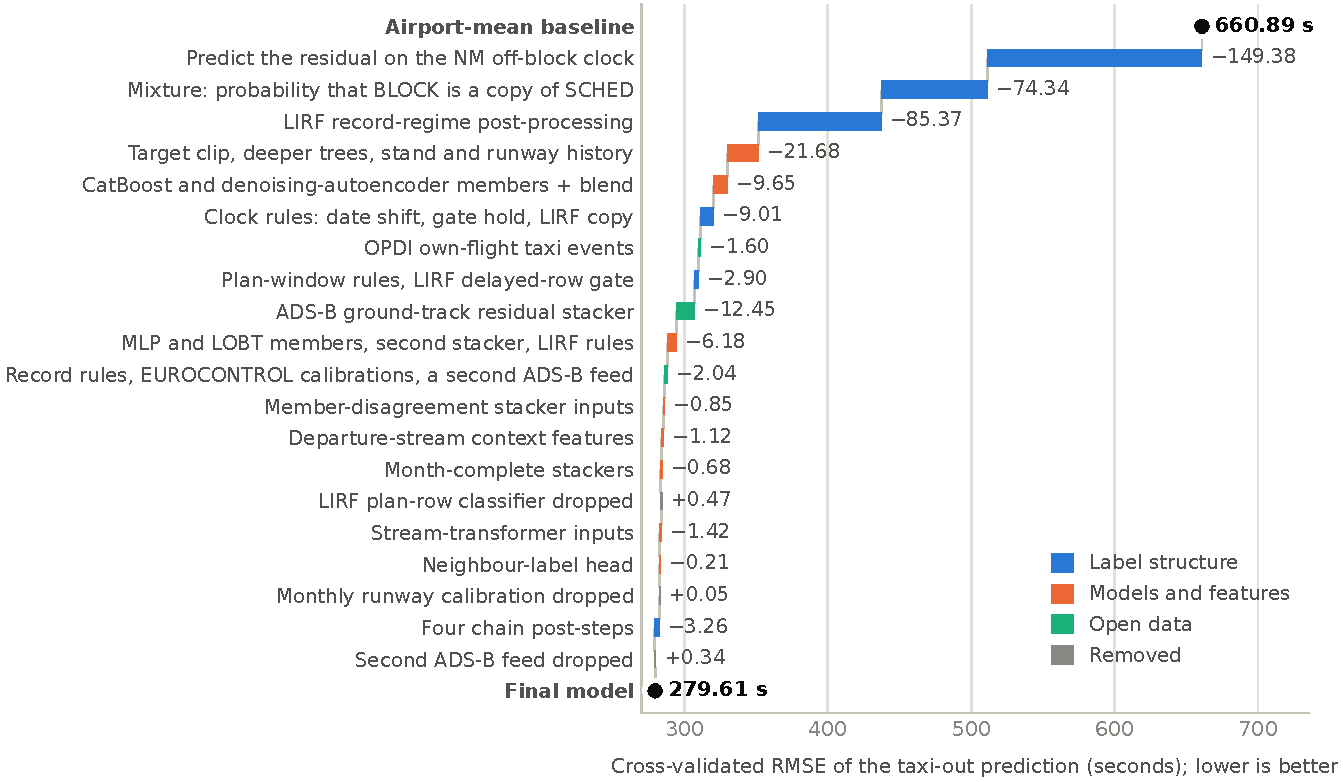
\includegraphics[width=\textwidth]{figures/fig-progress.pdf}
  \caption{From a 660.89\,s baseline to the final model, each bar one stage measured on the same two validation months. The three
  largest cuts (label structure) come from understanding the label; open data gives the largest later gain.}
  \label{fig:progress}
\end{figure}

On the twelve-month score weighted like the test months (Section~\ref{sec:twelve}), departure-stream context gains $-0.58$\,s
[$-0.76$, $-0.41$] with every month better, and month-complete stackers gain $-0.71$\,s [$-0.86$, $-0.56$] with 11 of 12 months
better.

\subsection{The chain step by step}

Table~\ref{tb:tail} and Figure~\ref{fig:tail} give each step after the rules chain against the one before. The stackers are worth $-3.48$\,s
here, against $-12.45$\,s for the first ADS-B stacker in Table~\ref{tb:progress}: that one corrected a chain with no ADS-B input at all,
while here five of the eleven members already read ADS-B features. Every interval lies below zero or ends at it.

\begin{table}[htbp!]
  \centering
  \small
  \caption{The reference chain step by step, RMSE (s). Each row adds one step to the rows above it. \emph{Trim} and \emph{clean} are the RMSE on trim and clean rows (Table~\ref{tb:terms}), \emph{Jan} and \emph{Jul} on each fold; \emph{Change} is the change in CV RMSE with a 95\% interval from the paired day-block bootstrap.}
  \label{tb:tail}
  \begin{tabular}{L{0.3\textwidth}rrrrrl}
  \toprule
  \textbf{Step} & \textbf{CV} & \textbf{Trim} & \textbf{Clean} & \textbf{Jan} & \textbf{Jul} & \textbf{Change [95\% CI]} \\
  \midrule
  rules chain on the blend & 292.33 & 230.30 & 217.47 & 326.80 & 261.27 & \\
  + ADS-B residual stackers & 288.85 & 225.85 & 212.72 & 323.25 & 257.81 & $-3.48$ [$-4.61$, $-2.69$] \\
  + LIRF no-plan copy classifier & 287.70 & 224.38 & 212.72 & 323.25 & 255.47 & $-1.15$ [$-2.62$, $-0.10$] \\
  + LIRF near-schedule rule & 287.25 & 223.80 & 212.77 & 323.32 & 254.49 & $-0.45$ [$-0.98$, $-0.07$] \\
  + LIRF plan-row copy classifier & 286.88 & 223.32 & 212.26 & 322.98 & 254.07 & $-0.37$ [$-0.69$, $-0.11$] \\
  + daily delay calibration & 285.75 & 221.83 & 210.77 & 322.49 & 252.27 & $-1.13$ [$-1.95$, $-0.53$] \\
  + duplicated-record rule & 285.47 & 221.47 & 210.59 & 322.12 & 252.08 & $-0.28$ [$-0.60$, $-0.07$] \\
  + monthly runway calibration & 285.44 & 221.44 & 210.54 & 322.11 & 252.03 & $-0.03$ [$-0.06$, $0.00$] \\
  \bottomrule
  \end{tabular}
\end{table}

\begin{figure}[htbp!]
  \centering
  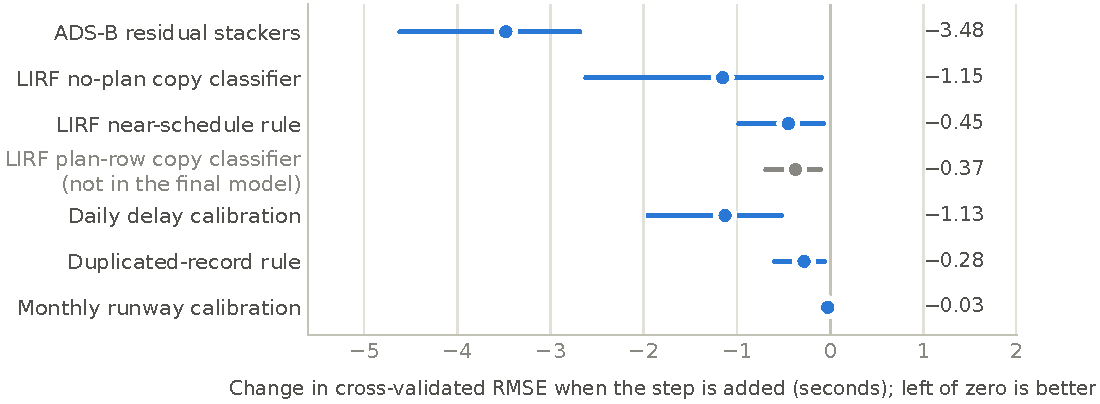
\includegraphics[width=0.9\textwidth]{figures/fig-tail.pdf}
  \caption{Each step after the rules chain against the one before, with its 95\% interval. The LIRF plan-row classifier (grey) is not in
  the final model.}
  \label{fig:tail}
\end{figure}

\subsection{By airport}

Paris and Rome hold two thirds of the squared error (Figure~\ref{fig:airports}, Table~\ref{tb:airports}). LFPG's January share is almost
entirely the two records of Section~\ref{sec:concentration}; LIRF's July error comes from its delayed departures without a flight plan.
On rows up to two hours the airports range from 79\,s (EDDM, January) to 505\,s (LIRF, July). On those rows the error is about 45\,s lower
where the aircraft's ADS-B track is known (188.3\,s for 182,684 matched rows against 233.1\,s for 161,735 unmatched), partly because of
the airport mix: LTFM and LFPG are mostly unmatched.

\begin{figure}[htbp!]
  \centering
  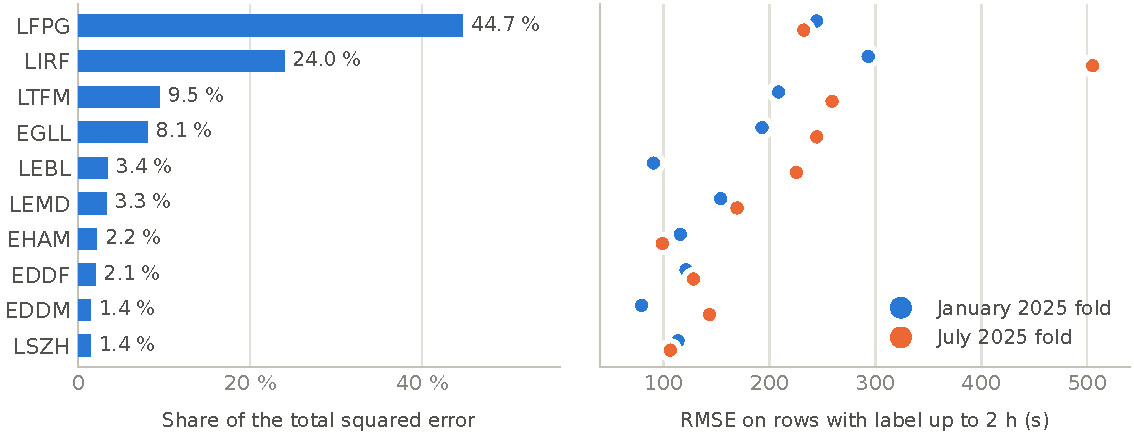
\includegraphics[width=\textwidth]{figures/fig-airports.pdf}
  \caption{Left: each airport's share of the squared error of both folds. Right: RMSE on rows with labels up to two hours, by fold.
  Paris and Rome hold two thirds of the squared error; on rows up to two hours every airport but Rome lies at 80--260\,s.}
  \label{fig:airports}
\end{figure}

\begin{table}[htbp!]
  \centering
  \small
  \caption{The reference chain by airport; each row is one airport. \emph{Rows} are validation departures, \emph{RMSE} is in seconds, $\le$2\,h excludes labels above two hours, \emph{ADS-B} is the share of departures with an ADS-B match and \emph{Share of SSE} is the airport's share of the total squared error.}
  \label{tb:airports}
  \begin{tabular}{lrrrrrrlr}
  \toprule
  \textbf{Airport} & \multicolumn{3}{c}{\textbf{January}} & \multicolumn{3}{c}{\textbf{July}} & \textbf{ADS-B} & \textbf{Share} \\
  & \textbf{Rows} & \textbf{RMSE} & \textbf{$\le$2\,h} & \textbf{Rows} & \textbf{RMSE} & \textbf{$\le$2\,h} & \textbf{Jan / Jul} & \textbf{of SSE} \\
  \midrule
  EDDF & 15,496 & 121.4 & 121.4 & 21,334 & 128.3 & 128.3 & 0.91 / 0.94 & 2.1\% \\
  EDDM & 11,266 & 79.3 & 79.3 & 15,825 & 143.5 & 143.5 & 0.97 / 0.37 & 1.4\% \\
  EGLL & 19,420 & 193.7 & 193.1 & 20,790 & 271.4 & 244.7 & 0.68 / 0.29 & 8.1\% \\
  EHAM & 18,460 & 141.1 & 115.9 & 22,489 & 104.3 & 98.9 & 0.99 / 0.98 & 2.2\% \\
  LEBL & 12,234 & 90.5 & 90.5 & 16,752 & 225.5 & 225.5 & 0.98 / 0.94 & 3.4\% \\
  LEMD & 16,510 & 154.0 & 154.0 & 18,818 & 169.5 & 169.5 & 0.00 / 0.30 & 3.3\% \\
  LFPG & 17,900 & 795.9 & 244.7 & 21,712 & 236.3 & 232.4 & 0.02 / 0.11 & 44.7\% \\
  LIRF & 11,317 & 372.8 & 293.3 & 15,211 & 582.0 & 505.3 & 0.01 / 0.94 & 24.0\% \\
  LSZH & 9,735 & 136.5 & 113.7 & 12,611 & 130.3 & 106.4 & 0.97 / 0.96 & 1.4\% \\
  LTFM & 21,368 & 213.0 & 208.7 & 25,171 & 259.2 & 259.2 & 0.00 / 0.00 & 9.5\% \\
  \bottomrule
  \end{tabular}
\end{table}

\begin{figure}[htbp!]
  \centering
  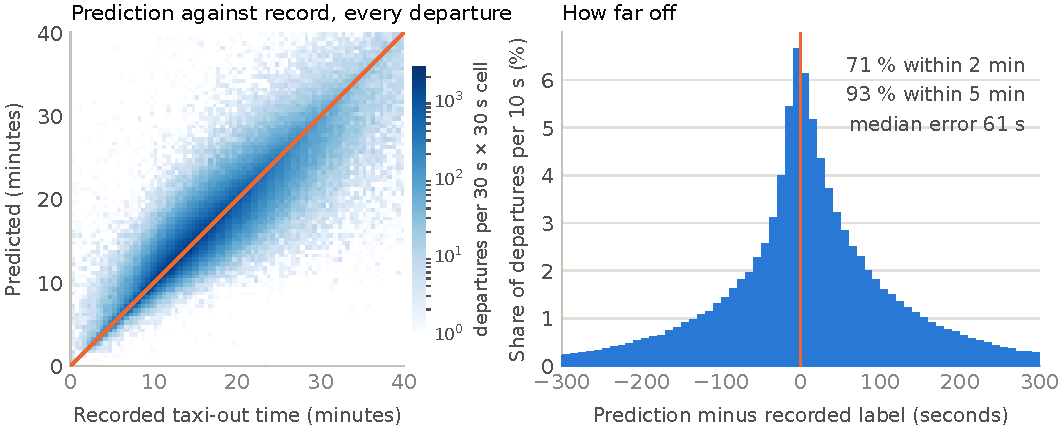
\includegraphics[width=\textwidth]{figures/fig-density.pdf}
  \caption{Predicted against recorded taxi-out time for the 344,419 departures of the January and July folds (final chain, out of fold). Left:
  departures per 30\,s $\times$ 30\,s cell on a logarithmic scale; the line is a perfect prediction; the 4,858 departures recorded at 40 minutes or more
  (1.4\% of the rows, 62\% of the squared error) lie outside the view. Right: prediction minus record, 10\,s bins; 71\% of the departures are within 2 minutes and 93\% within 5 minutes.}
  \label{fig:density}
\end{figure}

\subsection{Where the remaining error sits}
\label{sec:budget}

Scored with the final model on four held-out months of 2025 (671,292 departures, RMSE 260.01\,s; January and July from the rebuilt final model, February and June from the same model evaluated on the rehearsal months, which still carries the LIRF plan-row step and the monthly runway step), the squared error splits
by kind of row (Figure~\ref{fig:budget}). Date-stamped Rome records, giant labels and far schedule copies are 741 rows and hold
46.8\% of it; without them the RMSE would be 189.77\,s. The inputs do not say which flight is one, so the model can only hedge on these rows.
The ordinary rows, 99.8\% of departures, hold 42.0\%, and they are spread rather than shifted: the probability and taxi calibrations hold
within each label-size bin. What remains is a queue level shared by the flights of one airport within 15--30 minutes. It sits where open
ADS-B tracks are absent: ordinary rows at Istanbul, Paris Charles de Gaulle, Heathrow and Rome without a track hold 24.3\% of all squared
error. An oracle that adds to each departure the mean error of the other departures within $\pm 15$, $\pm 30$ or $\pm 60$ minutes would
cut the RMSE by 2.97, 2.90 and 2.49\,s; this is a ceiling, since it reads other flights' labels, and it is about one percent. It
is why the last model changes give each departure a view of its neighbours (the stream transformer) instead of adding per-row features.

\begin{figure}[htbp!]
  \centering
  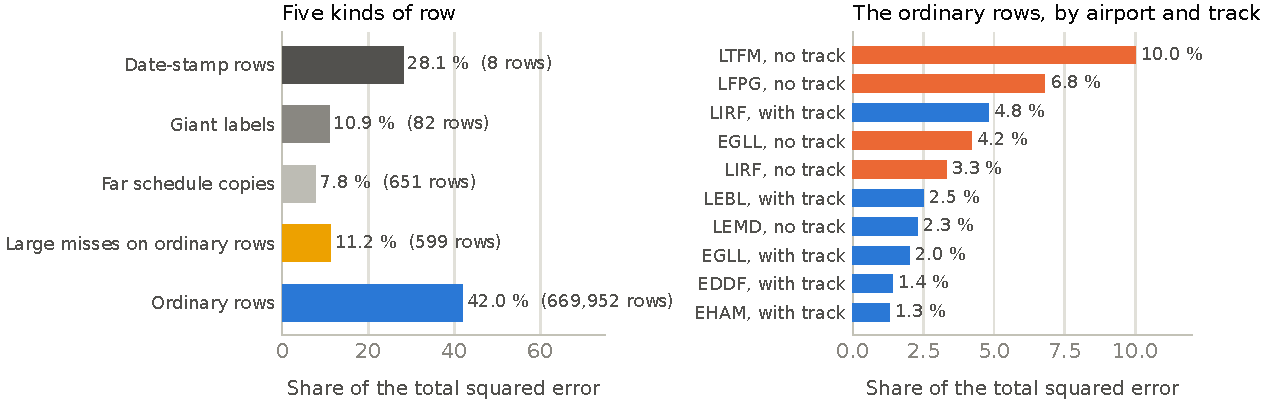
\includegraphics[width=\textwidth]{figures/fig-error-budget.pdf}
  \caption{Left: share of squared error by kind of row. Right: the ordinary rows by airport and ground track; the four orange bars
  are hubs without tracks and hold 24.3\% of all squared error.}
  \label{fig:budget}
\end{figure}

\subsection{By month}

A base mixture predicts each month of 2025 from the nine months that are neither that month nor its neighbours (RMSE 316.42\,s overall,
clean 207.29\,s). Figure~\ref{fig:months} splits its MSE by label regime. July is the hardest month (461.7\,s) and October the easiest
(210.9\,s). Copies are 4.6--6.2\% of departures in every month, but their cost peaks in summer: a missed copy costs about the square of
the flight's off-block delay, and delays peak in summer. Rows over two hours are heavy but erratic (January as large as July, November
above June).

\begin{figure}[htbp!]
  \centering
  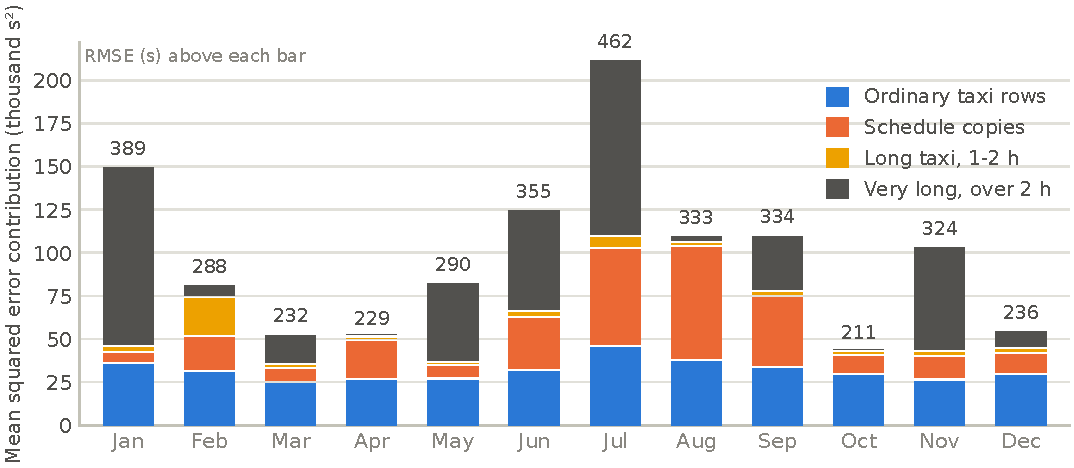
\includegraphics[width=0.9\textwidth]{figures/fig-months.pdf}
  \caption{Leave-one-month-out MSE of the base mixture by month and label regime; RMSE above each bar. Missed schedule copies drive the
  summer rise.}
  \label{fig:months}
\end{figure}

\subsection{Rehearsal on held-out months}

On the rehearsal (Section~\ref{sec:rehearsal}) the reference chain scores 247.48\,s (trim 201.81\,s, clean 191.54\,s; February 208.21\,s,
June 274.39\,s). The airport-mean baseline scores 558.74\,s on the same rows (February 606.14\,s, June 518.51\,s), against 660.89\,s on the
folds: these two months are easier than January and July, so 247.48\,s compares with 558.74\,s, not with the folds' scores. The final
model has no single rehearsal number, because its month-complete stackers learn from the held-out pairs; its additions are scored on the
twelve-month score instead. By airport (Figure~\ref{fig:rehearsal}) the pattern of the folds recurs: Rome, Istanbul in a snow month, then
Paris and Heathrow. The mean error on rows up to two hours is slightly negative ($-4.0$\,s overall), most at LTFM, EGLL, LEMD and LFPG.

\begin{figure}[htbp!]
  \centering
  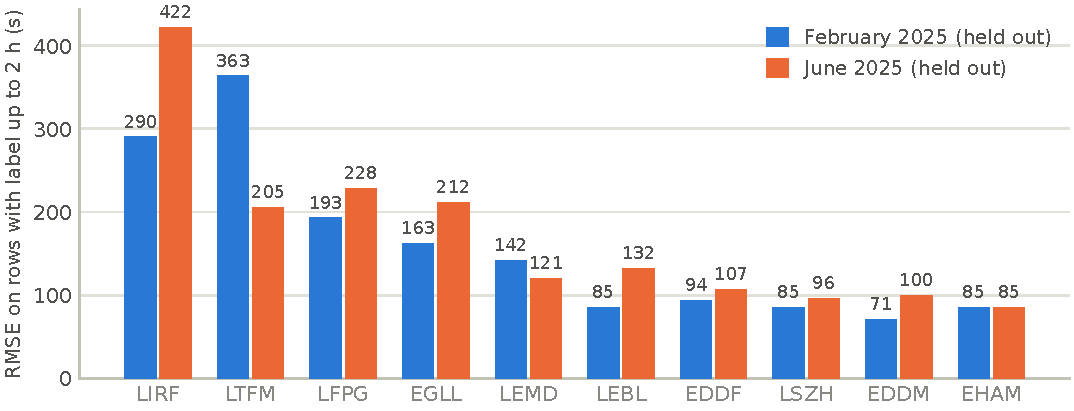
\includegraphics[width=0.9\textwidth]{figures/fig-rehearsal.pdf}
  \caption{Rehearsal on held-out February and June 2025: RMSE on rows up to two hours, by airport. February at LTFM is a snow month.}
  \label{fig:rehearsal}
\end{figure}

Table~\ref{tb:rehearsal} gives each step's effect on the two held-out months. The rules chain, the stackers and both calibrations gain in
both months (the final chain keeps only the daily one). The daily delay calibration's February gain is far larger than on the folds and very uncertain: a few days with heavy delays
carry it.

\begin{table}[htbp!]
  \centering
  \footnotesize
  \caption{Steps on the two held-out months of the February--June rehearsal. Each row is one step of the reference chain; each cell gives the RMSE (s) before $\to$ after the step and the change in MSE (s$^2$) with a 95\% interval.}
  \label{tb:rehearsal}
  \begin{tabular}{L{0.27\textwidth}L{0.31\textwidth}L{0.31\textwidth}}
  \toprule
  \textbf{Step} & \textbf{February 2025} & \textbf{June 2025} \\
  \midrule
  gate, plan cliff, plan-window clip & 238.88 $\to$ 236.47, $-1{,}145$ [$-2{,}144$, $-305$] & 283.93 $\to$ 276.16, $-4{,}351$ [$-7{,}285$, $-1{,}893$] \\
  ADS-B stackers & 236.47 $\to$ 227.71, $-4{,}069$ [$-6{,}815$, $-1{,}892$] & 276.16 $\to$ 274.54, $-894$ [$-1{,}017$, $-766$] \\
  LIRF no-plan classifier & no rows touched & 274.54 $\to$ 277.25, $+1{,}492$ [$-689$, $+5{,}375$] \\
  LIRF near-schedule rule & no rows touched & 277.25 $\to$ 276.85, $-219$ [$-566$, $0$] \\
  LIRF plan-row classifier (not in the final model) & 227.71 $\to$ 226.34, $-619$ [$-1{,}034$, $-211$] & 276.85 $\to$ 277.12, $+150$ [$+7$, $+300$] \\
  daily delay calibration & 226.34 $\to$ 208.33, $-7{,}829$ [$-18{,}433$, $-752$] & 277.12 $\to$ 274.89, $-1{,}233$ [$-3{,}068$, $-218$] \\
  duplicated-record rule & 208.33 $\to$ 208.27, $-28$ [$-105$, $+41$] & 274.89 $\to$ 274.49, $-219$ [$-489$, $-3$] \\
  monthly runway calibration & 208.27 $\to$ 208.21, $-25$ [$-34$, $-16$] & 274.49 $\to$ 274.39, $-52$ [$-64$, $-42$] \\
  \bottomrule
  \end{tabular}
\end{table}

\subsection{Calibration of the prediction}

Grouped by prediction, the mean error is small up to 30 minutes: $-6.6$\,s for predictions under 5 minutes, $+1.8$\,s at 5--10 minutes
and $-2.5$, $-4.1$ and $-6.9$\,s at 10--15, 15--20 and 20--30 minutes (Figure~\ref{fig:calibration}, left). Grouped by true value it shows
the regression to the mean expected of a conditional-mean model whose inputs cannot see why a taxi is long: $+418$\,s for the 79 rows with
$y \le 0$, $-251$\,s at 30--60 minutes, $-992$\,s at 1--2 hours and $-5{,}571$\,s above two hours (Figure~\ref{fig:calibration}, right).

\begin{figure}[htbp!]
  \centering
  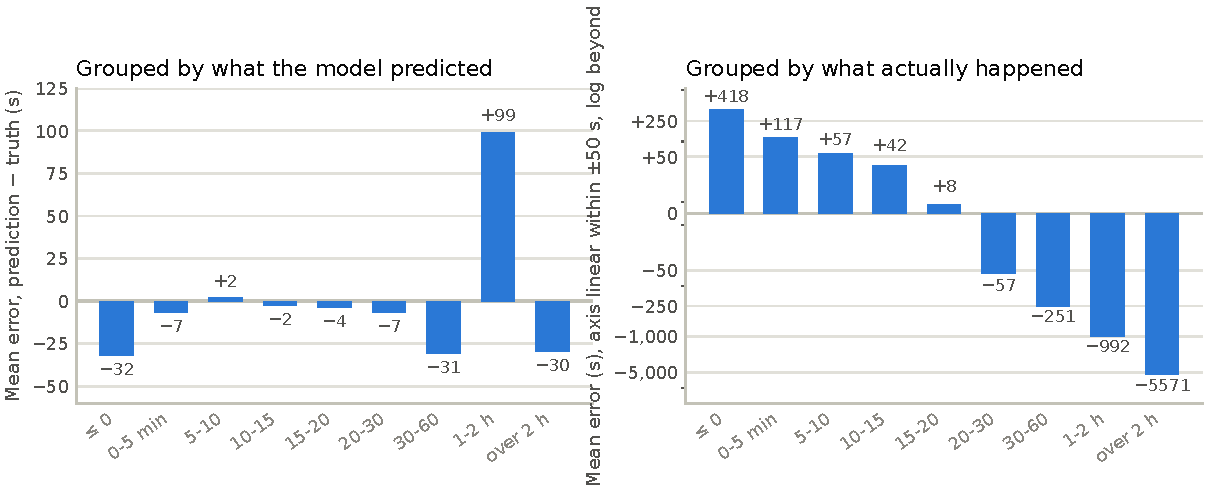
\includegraphics[width=\textwidth]{figures/fig-calibration.pdf}
  \caption{Mean error (prediction minus truth) grouped by the prediction (left) and by the true value (right). The model is right on
  average up to 30 minutes of prediction; long true taxis are predicted too short, as a conditional mean must when their cause is not in
  the inputs.}
  \label{fig:calibration}
\end{figure}


% ====================================================================================================================
\section{Discussion and limitations}
\label{sec:discussion}

\paragraph{The label decides most of the score.} The three largest gains came from reading what the label is (Table~\ref{tb:progress}):
a residual on an independent off-block clock, a mixture for schedule copies and airport-specific stamping regimes. Together they take
309\,s off the baseline; all members, stackers and open data after them take another 73\,s. The order matters beyond the challenge.
A model fitted to the raw label without separating the copies would learn delay propagation as if it were taxiing, and its estimates of
additional taxi time, fuel and emissions would inherit that bias. Because our model keeps $p$ and the physical taxi $r$ as separate
outputs, it can report which records are likely artefacts.

\paragraph{What did not help, and why.} Table~\ref{tb:negative} lists the alternatives we measured and left out. A positive
change is worse. Changes marked $^\dagger$ are CV RMSE (s) on the two folds against the model of the time (an earlier, weaker chain);
the others are against the final model.
\begin{table}[htbp!]
  \centering
  \small
  \caption{What did not help, and why. Each row is one method that was tried and left out; \emph{Change} is the change in RMSE (s)
  (positive: worse), with a 95\% interval where one was computed; $^\dagger$ see the text above.}
  \label{tb:negative}
  \begin{tabularx}{\textwidth}{@{}p{0.30\textwidth}p{0.20\textwidth}X@{}}
    \toprule
    Method & Change & Reason \\
    \midrule
    Gates and expert models that single out rows with huge errors$^\dagger$ & best $-3.2$ [$-15$, $+3.9$]; $+5.5$ on clean rows & They do not beat the conditional mean of Equation~\ref{eq:mixture}. \\
    Specialist for delayed schedule copies$^\dagger$ & $-0.2$ [$-1.2$, $+0.7$] & A tie with the mixture. \\
    Per-airport blend weights (NNLS or least squares)$^\dagger$ & $+1.04$ (NNLS), $+0.92$ (least squares) on trim rows & Worse than one global set of weights. \\
    Raw flight numbers and callsigns as features & not scored as a change & They carry most of the drift between years (Section~\ref{sec:drift}). \\
    Calibrating the copy probability per cell (no plan $\times$ local date change $\times$ delay bin)$^\dagger$ & $+1.8$ to $+11.5$ & Copies stay flat from month to month while real delays grow in summer, so rates measured in other months mislead. \\
    LIRF plan-row copy classifier & $-0.37$ [$-0.69$, $-0.11$] on the folds; $-0.09$ [$-0.23$, $+0.04$] over six rehearsal pairs & Gains on the folds and in February 2025, loses in June 2025 with an interval that excludes zero; neutral overall, so the final model drops it. \\
    Monthly runway calibration & $-0.03$ on the folds; $-0.028$ [$-0.046$, $-0.010$] over twelve months & A small gain that needs a second published aggregate of the scored months; left out so that the model uses one. Without a guard on the invalid-flight share it loses 150\,s$^2$ of MSE at LTFM in the February 2025 snow month (invalid flights were 0.111 of that month against at most 0.002 in every other month). \\
    Target encodings of nine keys$^\dagger$ & $+2.6$ (clean rows) & Worse on clean rows. \\
    \bottomrule
  \end{tabularx}
\end{table}
In the other direction, among the open data, removing OPDI from every member costs 0.51\,s of CV RMSE. A second ADS-B feed
without an open licence, read by earlier versions, was worth 0.30\,s on twelve months; the final model leaves it out.

\paragraph{Labels with no warning.} The two LFPG records of Section~\ref{sec:concentration} hold 36.5\% of the cross-validated squared
error. Seven of the 77 rows above 20,000\,s in 2025 are like them. Any test month may contain a few, and they move its RMSE by more than any
modelling choice. Every score here includes them.

\paragraph{Long genuine taxis are shrunk.} Rows that truly took one to two hours are predicted about 990\,s too short, and rows above two
hours about 5,600\,s too short. The inputs rarely show why a taxi is long (a remote hold, a de-icing queue, a closed runway), so the
conditional mean stays near the ordinary taxi. That is the right answer under squared error and a poor estimate of those rows.

\paragraph{Rome.} LIRF holds 24\% of the cross-validated squared error. Its copy classifiers' AUC stops near 0.88--0.91: copies of delayed
flights depend on the handler and the day in ways no available field fully records. The LIRF no-plan classifier is the weakest step that
stays: neutral over the six held-out pairs ($-0.01$\,s, better in 4 of 6) and a loss in June 2025 with an interval that includes zero
(Table~\ref{tb:rehearsal}). It acts only on ADS-B-matched LIRF rows, which in the test months are mostly January and February 2026 (77\%
and 70\% matched against 0\% in the same months of 2025), so no validation month resembles them.

\paragraph{Coverage holes in the open sources.} Open ADS-B ground coverage varies sharply by airport and month (Figure~\ref{fig:coverage}).
LTFM has almost none (under 1\%) and LFPG 1--33\%, so the stackers can only use clocks there. EDDF fell from 91--98\% in every 2025 month to
73--76\% in January, June and July 2026 and 26\% in February 2026 in the source's own daily files, for an unknown reason. If each of the
roughly 10,000 EDDF departures of February 2026 that lack a match lost the whole stacker gain measured on matched EDDF rows (MSE 14,015 to
11,780\,s$^2$), the test RMSE would rise by at most about 0.07\,s. LEMD and EGLL are far better covered in 2026 than in the same months of
2025; LIRF in June and July 2026 far worse. OPDI events are almost absent at EDDM from 21 January to 19 February 2026 (20\% of departures
against 84\% a year earlier); the effect of that gap is not measured.

\begin{figure}[htbp!]
  \centering
  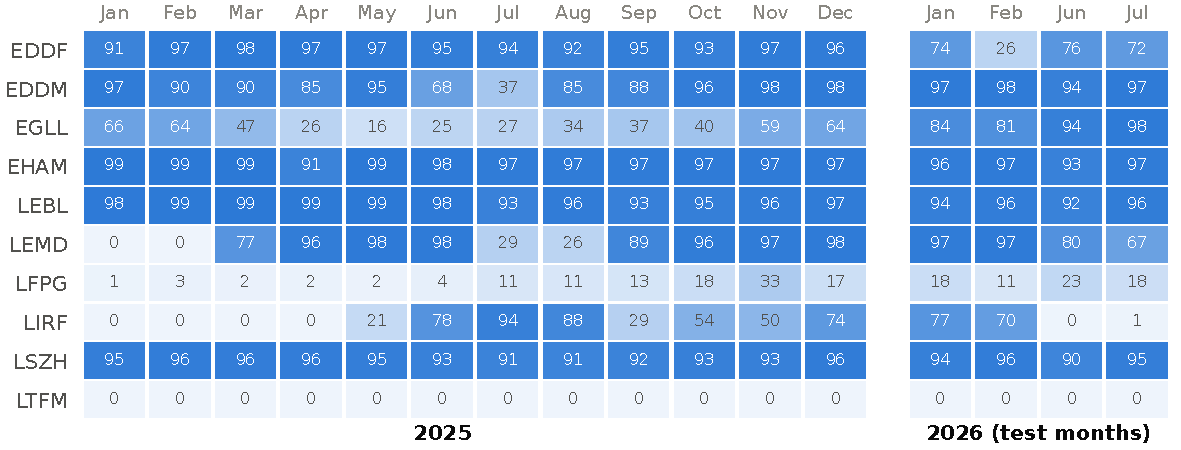
\includegraphics[width=\textwidth]{figures/fig-coverage.pdf}
  \caption{Share of departures with an ADS-B match, by airport and month, in 2025 and in the 2026 test months. Istanbul and Paris are
  almost never seen on the ground; Madrid, Heathrow and Rome switch between years.}
  \label{fig:coverage}
\end{figure}

\paragraph{Dependence on published aggregates and on the post-operations setting.} The daily calibration needs EUROCONTROL to have
published the daily delay for the scored days; a day without a value stays unchanged. The daily total is an aggregate of the outcome
on the scored days. The challenge's model is for post-operations use, where EUROCONTROL publishes that total for every day the model
is applied to (all 1,200 scored airport-days have one), so the step uses what the model has in its intended use. In tactical use the
total would not exist, and the step is switched off (\texttt{TAIL\_SKIP=dlyh} in the tail script \texttt{overnight/tail\_chain.sh}) at
a cost of 0.72\,s RMSE on twelve months and 1.41\,s on the January/July CV, both measured on an earlier version of the chain. The arrival-side copy habits and the stand histories also
read records after the movement, which a real-time system could not do.

\paragraph{Validation optimism.} The members early-stop on the folds' non-copy rows, rule thresholds were set on 2025 data including
the folds, the month-complete stackers score each fold month by day-blocks (other days of the month are in training), the LIRF no-plan
classifier and the post-step pool keep the fold's neighbouring months in training (with them left out the classifier's gain falls from
1.23 to 0.47\,s), and many runs were compared on the same two folds. The rehearsal and the twelve-month score check months those comparisons did
not use, and the rehearsal is itself an upper bound (Section~\ref{sec:rehearsal}).

\paragraph{The public leaderboard.} The public leaderboard scores the same January and July 2026 rows on every submission, so
each score is an exact equation in the hidden labels and repeated submissions decode single labels. We probed the board from
29 September to 12 October. The probes confirmed the mechanism on the board first, so the private note we sent the organisers on
3 October reported a measured effect, with a fix: rank the final on labels the board never scores. Five days later, on 8 October, the
organisers added blind February and June months to the final ranking. On 13 October a board-only file, the shipped final's
January/July predictions with 91 rows replaced by decoded labels, scored 208.11\,s RMSE and ranked first, which shows the size.
The shipped final has nothing to do with the probing: it contains no decoded label, and the code has no probe or decode step.
None of this needs checking from the code: the final is also scored on blind February and June 2026, which no board submission
ever touched, and that score is the check. It measures the model plus the published daily delay calibration, which runs on those
months too (rehearsal, reference chain: February 226.34\,s before that step and 208.33\,s after, June 277.12\,s and 274.89\,s).

\paragraph{Reproducibility of numbers.} GPU CatBoost is not bit-reproducible: two single-seed runs of the delayed-row gate differ by about
$\pm 0.1$\,s of CV RMSE, so the gate averages five seeds (285.40\,s instead of 285.44\,s for the reference chain). Each change in the
tables compares two runs on the same upstream draw, so the draw cancels in it. Every other fitter is seeded; a replay of the chain stage
from the same inputs reproduces every file up to the blend bit for bit.


% ====================================================================================================================
\section{Conclusion}
\label{sec:conclusion}

For about one departure in twenty, predicting taxi-out time from airport records means predicting how the record was made. Most of
the error reduction from 660.89\,s to 279.61\,s comes from treating the label as a mixture of a physical taxi and a schedule copy,
with a calibrated copy probability, and from encoding the other ways the record goes wrong as measured rules. Open ADS-B tracks and
published aggregates add smaller, consistent gains, and a validation design built for unlabelled months of a later year checks each
step on months it was not tuned on. Records whose errors nothing in the data announces dominate what remains. For performance
monitoring, taxi-out statistics built from recorded off-block times should first separate copied stamps from events; the copy
probability does that per flight.

The released code can be extended as well as replayed. A new set of months needs the final-phase stages only, since the 2025
members, the rehearsals and the base of the month-complete stackers are reused. The calibration to the published daily delay can be
switched off at the cost given in Section~\ref{sec:discussion}. A new feature family is one script that writes one file with a row per
departure, picked up by name by the members and the stackers. A member can join through its disagreement with the eleven, without
changing the blend. Each recipe, the files to edit for another airport, the checks (a paired comparison, a month-weighted comparison and a
synthetic-data smoke run) and the hardware and time per step are in the repository's \texttt{docs/extending.md}.


\paragraph{Reuse in OPDI.} Three steps need only the actual off-block time (AOBT), the actual take-off time (ATOT), the scheduled time and
an ADS-B ground track, all of which the open flight-event tables of OPDI \cite{goens2024opdi} can supply. (i) Copy detection: a record whose
off-block time equals the schedule to within 30\,s (the label's \fld{BLOCK} against \fld{SCHED}) is flagged as a stamp, not an event, and
the copy probability of Section~\ref{sec:mechanisms} estimates it where the record is unknown. (ii) The physical taxi: take-off minus the
off-block time, on the rows whose record is an event. The members regress the residual of that quantity on an anchor (the Network Manager's off-block time or the last filed one) and take the
ADS-B first movement and ground events as inputs, not as the target: the first movement lies a median $-1$\,s (EHAM) to $+758$\,s (LFPG) from the recorded off-block, within a minute for more than half the departures only at EDDM and EHAM (\texttt{docs/extending.md}, ``Notes on what was measured''). (iii) Plausibility screens before taxi-out statistics are built: durations outside 0--3,600\,s and
take-offs far from the off-block time are set aside as in Section~\ref{sec:checks}. Field names do not carry their units in the code (\fld{a2\_gs1} is seconds; the units are in \texttt{docs/extending.md} and \texttt{docs/features.md}); a port to OPDI would put the unit in the name.

\section*{Acknowledgement}
The author thanks the EUROCONTROL Performance Review Commission and Performance Review Unit for organising the Data Challenge and
publishing its data, and the communities behind adsb.lol, OpenStreetMap, OurAirports and the Iowa Environmental Mesonet
for open data.

\section*{Authorship and AI assistance}
This work was AI-assisted, with Anthropic's Claude (through Claude Code) and OpenAI's Codex.

\section*{Funding statement}
No external funding. The computations ran on the author's own hardware; only free tiers of cloud notebooks were used besides.

\section*{Open data statement}
The challenge data (2025 training files and 2026 test files) are provided by the EUROCONTROL Performance Review Commission through the
PRC Data Challenge 2026 \cite{prc2026challenge} and are not redistributed with this paper. All external inputs are publicly accessible
from the sources of Table~\ref{tb:sources}, each under its own terms (not all are open licences): adsb.lol (Open Database Licence), the METAR archive of the Iowa Environmental Mesonet, EUROCONTROL Performance Review data and OPDI (use with
attribution of EUROCONTROL as source), OpenStreetMap (Open Database Licence) and OurAirports (public domain). The small tables behind
every figure and every number in this paper (by stage, airport, month and calibration bin) are in the \texttt{writeup/data/} directory of
the accompanying repository.

\section*{Reproducibility statement}
The pipeline code is in the \texttt{code/} directory of the repository that accompanies this paper, under
the GNU General Public License v3. It runs as one shell script per stage (data, features, members, chain, test months, prediction file),
records the parameters and cross-validated score of every step as one JSON file in \texttt{code/recipes/}, and includes a CPU smoke test
that runs every stage up to the bundle chain on small synthetic data. The figures of this paper are drawn by \texttt{paper/make\_figures.py} from
\texttt{writeup/data/*.csv}; every table is taken from the same files or from the documentation in \texttt{docs/}. Hardware: one CUDA GPU
for the members (about five GPU-hours for the two folds and the test refits) and a multi-core CPU with 16\,GB of memory or more for
features and stackers.

\printbibliography

\end{document}
